\chapter{Evaluation}\label{ch:evaluation}
% take a step back and put your results from 4 into context.
This chapter represents the evaluation phase, which includes the evaluation, demonstration and
communication activities outlined in the \ac{DSR} process in \cref{ch:research-methodology}.

The evaluation activity provides a comprehensive analysis of the Machine Learning models built in the
previous chapter.
This phase evaluates the effectiveness of the developed models in solving the defined research questions.
During the demonstration phase, different scenarios are chosen to illustrate the potential real-world applications of
the of the models and their performance in these contexts.
Finally, during the communication phase, the results of this study will be presented with the aim of effectively
communicate the results and their interpretation.

\cref{tab:evaluation_criteria} provides an overview of the quality metrics employed for the evaluation,
structured based on the \ac{GQM} approach discussed in \cref{sec:goal-question-metric-approach}.
The quality metrics align with the quality model from~\cite{siebert2022construction}, which in turn is based on
the ISO/IEC 9126 standard for software quality evaluation.
This standard has been adapted by\cite{siebert2022construction} to address the specific requirements of machine
learning models, as detailed in Section~\ref{sec:evaluation-of-machine-learning-models}.
Since~\cite{siebert2022construction} primarily focus on evaluating classification models, the quality metrics have
been tailored to suit the needs of the regression models implemented in this study.
Each individual quality metric section provides further elaboration, on what was changed.
\cref{tab:evaluation_criteria} also displays the quality metrics used for evaluating the \ac{ML} models.

\captionsetup{margin={5pt,5pt}}
\begin{table}[H]
    \begin{tcolorbox}[arc=0pt,boxrule=0.5pt]
        \centering
        {\renewcommand{\arraystretch}{1}
            \begin{tabular}{p{2cm}p{8cm}p{3cm}}
                \toprule
                \thead{\textbf{Goal}} & \thead{\textbf{Question}}
                & \thead{\textbf{Metric}} \\
                \toprule
                \textbf{Correctness} &
                How is the ability of the model to perform the current task measured on the development dataset and
                the runtime dataset
                ~\cite[p. 16]{siebert2022construction}?
                &
                MAE, \newline MSE, \newline RMSE
                \\
                \hdashline
                \textbf{Relevance} &
                Does the bias-variance tradeoff work well for the model? which means that the data should not be
                overfit or underfit.
                ~\cite[p. 16]{siebert2022construction}?
                & Variance of CV, \newline $R^2$
                \\
                \hdashline
                \textbf{Robustness} & Ability of the model to outliers, noise
                and other data quality issues~\cite[p. 16]{siebert2022construction}
                & Loss of Accuracy, \newline Average Loss
                \\
                \hdashline
                \textbf{Stability} & Does the artifact generate repeatable
                results when trained on different data?~\cite[p. 16]{siebert2022construction}
                & LOOCV stability
                \\
                \hdashline
                \textbf{Interpret- ability} & How well can the model be
                explained?~\cite[p. 16]{siebert2022construction}
                & Linearity, \newline monotonicity, \newline  interaction
                \\
                \hdashline
                \textbf{Resource utilization} & How much resources are
                required to train and run
                the model?~\cite[p. 16]{siebert2022construction}
                & Training time, \newline runtime, \newline storage space
                \\
                \bottomrule
            \end{tabular}
        } % renew command
    \end{tcolorbox}
    \caption{Overview of the goals, questions and metrics for the
    evaluation of artifacts
    following the \ac{GQM} approach.}
    \label{tab:evaluation_criteria}
\end{table}


\section{DP1: Correctness}\label{sec:dp1:-correctness}
% Ability of the model to perform the current task measured on the
% development dataset and the
% runtime dataset

The model must be able to perform well on the selected task.
\cite{siebert2022construction} used the classification metrics precision, recall and F- score to evaluate the
correctness.
Since predicting the spring back is a regression task, these metrics are not applicable.
For this study metrics are needed to measure how well the predicted spring back for a specific observation
matches the actual spring back~\cite[p. 29]{hastie2009elements}.
These metrics used in this study are the MAE, MSE and RMSE and where presented in~\cref{subsubsec:regression-metrics}
For the evaluation the \textit{sci-kit learn}~(\cite{scikit-learn}) implementations of these metrics were used.

There is an ongoing debate regarding the best metric to use for evaluating regression models.
For instance~\cite{willmott2005advantages} contend that the RMSE is not an appropriate measure for determining the
average performance of a model and suggest using the MAE instead, while~\cite{chai2014root} argue in favor of the RMSE.
The MAE is commonly used when a dataset contains outliers.
However, as the dataset reviewed in \cref{subsec:dataset-exploration} is likely to not contain many outliers, the
RMSE will be used as the primary metric in this study~\cite[p. 1249]{chai2014root}.
The MSE and MAE will be used as well but only when they make sense, for example when noise is added to the dataset
and therefore more outliers (\cref{sec:robustness}) are present or if the non squared error yields more meaningful
results.

Both measures will be included in the analysis, to give the reader a better understanding of the performance of
the models.
The MSE was not included in the analysis, as it is not expressed in the same unit as the data and is therefore
more difficult to interpret and might be misleading.

\subsection{Results}\label{subsec:results}
\cref{tab:results-correctness} presents the results of the evaluation of the Machine Learning models for
correctness, sorted by the RMSE in ascending order.
It can be can be concluded that the best models have an RMSE of less than 0.2 millimetres, indicating that they can
predict the spring back with acceptable accuracy for many applications.

The Linear Regression and Decision Tree models have poor predictive performance compared to the other models.
For the \ac{LR} model this is expected since the relationship between the independent and dependent variables is
not linear.
In contrast, Decision Trees can perform poorly when overfitting the training data and they are prone to
instability.
These problems are mitigated by using ensemble methods like Random Forest and Gradient Boosted Treesj.
As the simple Decision Tree and Linear Regression models are not able to predict the spring back accurately enough,
they are not considered for the next steps of the evaluation.
The Ada Boost, Random Forest, and Gradient Boosted Tree models demonstrate moderate predictive
performance while the Multi-Layer-Perceptron, Extra Trees, and Support Vector Machine models have relatively low MAE
and RMSE values, indicating good predictive performance.

It is worth noting that the SVM model has a slightly better MAE while still maintaining a comparable RMSE compared
to the other models.
This could be because the errors made by the SVM are evenly distributed across instances or
because the errors made by the other models are large for a few instances but smaller for the rest.

% Table wit hall used machine learning models and their metrics
\begin{table}[H]
    \begin{tcolorbox}[arc=0pt,boxrule=0.5pt]
% \sisetup{group-minimum-digits = 4}
        \centering
        \begin{tabular}{lll}
            \toprule
            \thead{\textbf{Model Name}} & \thead{\textbf{MAE}}
            & \thead{\textbf{RMSE}} \\
            \toprule
            \textbf{Decision Tree}            & 0.255 & 0.348 \\
            \hdashline
            \textbf{Linear Regression}        & 0.220 & 0.282 \\
            \hdashline
            \textbf{Ada Boost}                & 0.202 & 0.261 \\
            \hdashline
            \textbf{Gradient Boosted Trees}   & 0.168 & 0.221 \\
            \hdashline
            \textbf{Random Forest}            & 0.159 & 0.221 \\
            \hdashline
            \textbf{Multi-Layered-Perceptron} & 0.136 & 0.190 \\
            \hdashline
            \textbf{Extra Trees }             & 0.135 & 0.172 \\
            \hdashline
            \textbf{Support Vector Machine}   & 0.106 & 0.146 \\
            \bottomrule
        \end{tabular}
    \end{tcolorbox}
    \caption{\textbf{Results for the Design Principle 1 Correctness:} The results are sorted by RMSE in ascending
    order.}
    \label{tab:results-correctness}
\end{table}

The overall performance of the machine learning modes are good and the best performing models are the Extra Trees and
Support Vector Machine models.


\section{DP2: Relevance}\label{sec:relevance}
% Does the model achieve a good bias-variance tradeoff? Which means neither
% overfitting or
% unterfitting the data.

% Bias variane trade-off
A model is considered relevant when it achieves a balance between bias and
variance, avoiding both overfitting and underfitting of the training data.
The relevance of the model can be quantified through the \textit{variance of cross-validation}, which proves insight
into how the model performs when trained and
evaluated on different subsets of data and how well it generalizes.

% Explanation interpretation of variance
A low variance indicates that the model's performance is consistent across
different folds, suggesting that the model is not overfitting the training data.
Conversely, a high variance implies that the performance can vary significantly
depending on the specific data points used in the test set, indicating a potential
overfitting problem.

A common metric for gauging the effectiveness of regression models is the $R2$ statistic, it shows how much of the
the variance is explained by the model.
It ranges usually from 0 to 1, where 0 means that the model doe not explain any of the variance and a score of 1
means that the model fully explains the variance
~\cite[p. 43]{muller_introductionmachinelearning_2016}.

\cref{eq:r2} shows the formula for the $R^2$ score as explained by
~\cite[p. 43]{muller_introductionmachinelearning_2016}.

\begin{equation}
    \label{eq:r2}
    R^2 = \frac{\text{Explained variance}}{\text{Total variance targert variable}}
\end{equation}

One unique feature of scikit-learn's implementation of $R^2$ is that the score can be negative if the model performs
poorly.
For instance, a model would receive a $R2$ score of 0.0 if it consistently predicted the expected value of y
regardless of the input features
~\cite{_sklearnmetricsr2_}.
Therefore, a high $R^2$ score indicates a good model fit and a good bias-variance
tradeoff~\cite[p. 43]{muller_introductionmachinelearning_2016}.

\subsection{Results}\label{subsec:results3}

\cref*{tab:results_relevance} displays the variance of cross-validation and the $R^2$ for all the machine
learning models used, sorted in ascending order of their $R^2$ score.
The variance of cross-validation was calculated using Scikit-Learn's \texttt{cross\_val\_score} method, and five
-fold cross-validation was used for the calculation.
The formula shown in \cref{eq:r2} was used to calculate the $R^2$ score.

It can be observed that most of the models have relatively low variance, indicating that their performance is
consistent across different folds.
Based on the table the following models have the best bias-variance tradeoff:

\begin{enumerate}
    \item Extra Trees: With an $R^2$ of 0.889 and a Variance of CV of 0.031, this model performs the best among
    the listed models. It has a high $R^2$ value, meaning it can explain a significant proportion of the
    variance in the data, and a relatively low Variance of CV, indicating stable performance across different
    subsets of the data.
    \item Multi-Layer Perceptron (MLP): The MLP model has the second-highest $R^2$ value of 0.825 and a low Variance
    of CV of 0.023, which implies that it can explain a substantial amount of variance in the data and perform
    consistently across different subsets.
    \item Random Forest: The Random Forest model has an $R^2$ value of 0.784 and a Variance of CV of 0.041.
    Although the model explains less variance.
\end{enumerate}

To gain a more full picture of how well your model is performing, evaluate the cross-validation scores in conjunction
with the other metrics.
This will be addressed in subsequent parts.


\begin{table}[h]
    \begin{tcolorbox}[arc=0pt,boxrule=0.5pt]
        \centering
        \begin{tabular}{lll}
            \toprule
            \thead{\textbf{Model Name}} & \thead{\textbf{Variance of CV}}
            & \thead{\textbf{$R^2$}} \\
            \toprule
            \textbf{Support Vector Machine} & 0.016 & 0.893 \\
            \hdashline
            \textbf{Extra Trees}            & 0.031 & 0.889 \\
            \hdashline
            \textbf{Multi-Layer-Perceptron} & 0.023 & 0.825 \\
            \hdashline
            \textbf{Random Forest}          & 0.041 & 0.784 \\
            \hdashline
            \textbf{Gradient Boosted Trees} & 0.021 & 0.761 \\
            \hdashline
            \textbf{Ada Boost}              & 0.072 & 0.676 \\
            \bottomrule
        \end{tabular}
    \end{tcolorbox}
    \caption{Performance of the used machine learning models according
    relevance.}
    \label{tab:results_relevance}
\end{table}


\section{DP3: Robustness}\label{sec:robustness}
% Definition of robustness

Unlike \ac{DP} Correctness(\cref{sec:dp1:-correctness}), robustness is a non-functional characteristic of a \ac{ML}
model.
A way to evaluate the robustness is to check the correctness of the model with added noise to the
data
~\cite[p. 1]{saez_evaluatingclassifierbehavior_2016}, if the model is still able to predict the correct values, it is
considered robust.
As mentioned in \cref{subsec:dataset-exploration} the data set was generated in a controlled environment does not
contain many data quality issues and noise as they where removed during the process.
This offers the opportunity to test the robustness of the models by manipulating the data set to introduce the data
quality issues missing values and noise.
To do that two tests where developed and are described in the following sections.

\subsection{Missing Data}\label{subsec:missing-data}
When applying the model to real-world data, it is possible that some values are missing.
Looking at the available dataset two scenarios or missing data can occur:
Missing $Vt$-pairings and missing values.

In the first scenario, there may be no data available for a specific die opening, which can be due to the die opening
was never being used before or a lack of recorded information.
In the second scenario, while data may exist for the desired $Vt$ combination, certain values may
be missing or the dataset may not be complete.

To address these scenarios, the following tests were conducted:

\subsubsection{Missing values}

Initially, the use of the \ac{LPOCV} method was considered.
However, this approach was omitted due to computational constraints, as it generates all possible
training and test sets by removing $p$ samples from the complete dataset, resulting in a large
number of overlapping test sets and a high computational cost.
As an alternative, regular \ac{CV} was applied, with an increasing number of folds.
The minimum number of folds was 2 and the maximum was equal to the total number of samples in the
dataset.
However, this experiment did not provide distinguishable results and was therefore not
included in the results.

The third and final experiment utilized random sampling to create different train-test data compositions, allowing
for the evaluation of the model's handling of missing data.
Split ratios from 90:10 to 10:90 were used, with a step size of 10.
This approach was inspired by a similar method used in a previous study~\cite[p. 570--574]{liu2021deep}  which used
thee different split ratios to evaluate the performance of a deep learning model.

The results of this experiment provided valuable insights into the model's performance under
different data compositions, particularly when dealing with missing
data, and were used in conjunction with other metrics to gain a comprehensive understanding of
the model's overall performance.

\cref{fig:results-missing-values} shows how the models performed when trained on
continuously less data.
It can be seen that all models perform well when trained with on 90\% of the data.
However, when trained on 50\% of the data, the \ac{MLP}  and \ac{GBT} models start to perform
better than the other models.
When trained on 20\% of the data and less all models significantly underperform.
Also the \ac{ET} model stays relatively stable when trained on less data.

\begin{figure}[h]
    \begin{tcolorbox}[arc=0pt,boxrule=0.5pt]
        \centering
        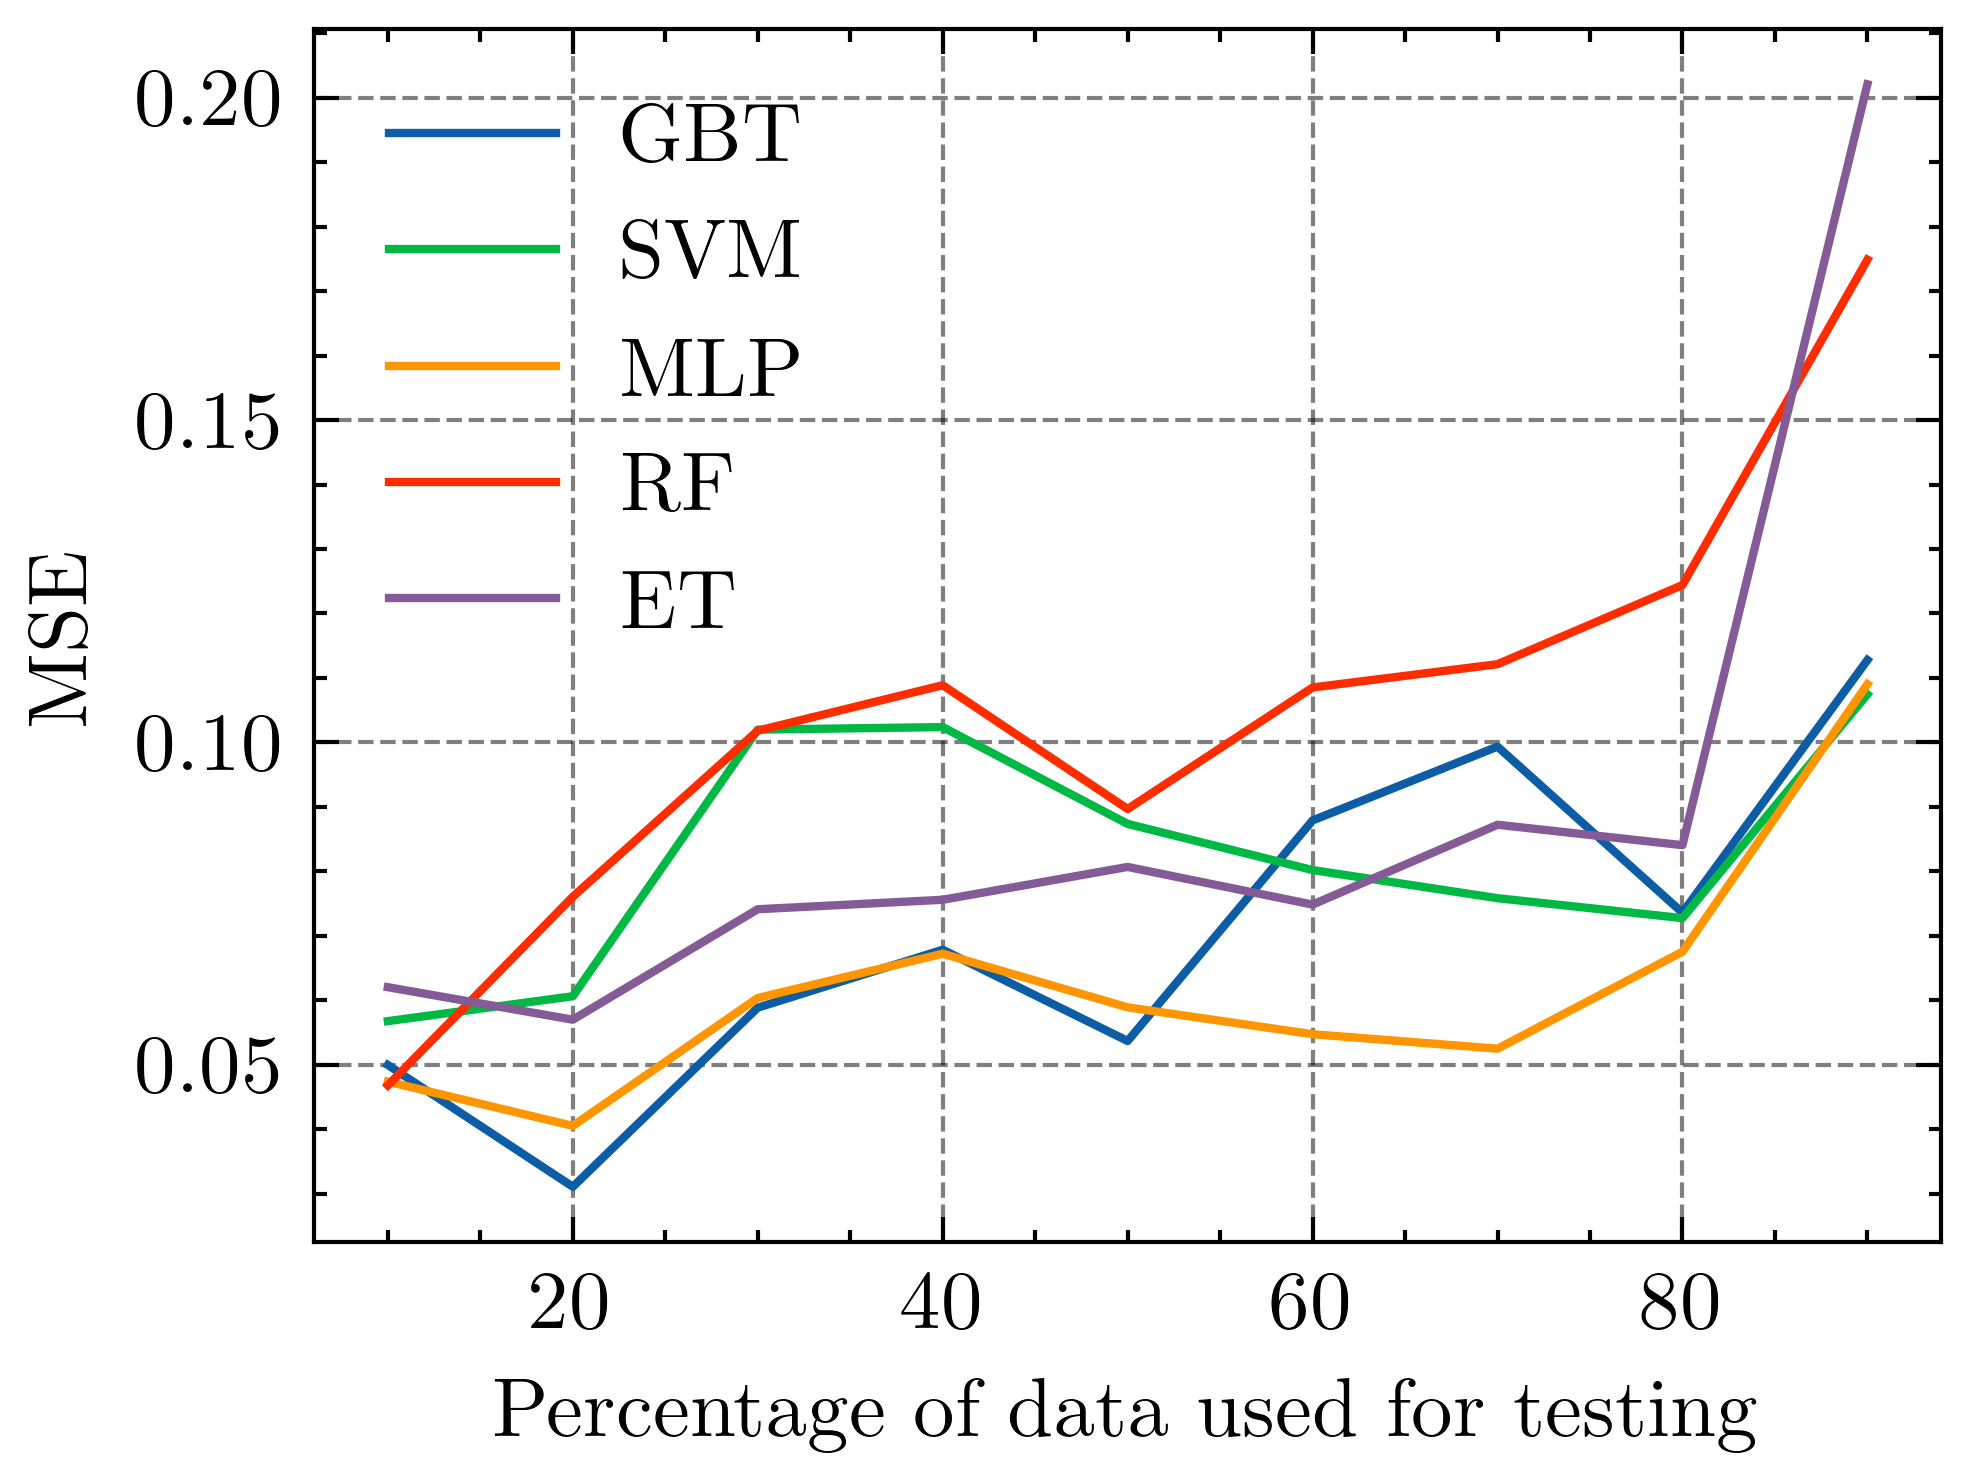
\includegraphics[width=0.6\textwidth]{chap5/images/missing_values_plot}
    \end{tcolorbox}
    \caption{Comparison of performance on less training data.}
    \label{fig:results-missing-values}
\end{figure}

Looking at the variances show in Figure~\ref{fig:variance-missing-values} the the \ac{SVM} and \ac{MLP} models
perform the best and seem to be the most robust models when trained on less data.
It has to be noted, that as seen in the previous figure the most variance comes from training on
below 20\% of the data.

Overall the \ac{MLP} model seems to be the most robust model, as it performs well on all data
compositions and has the lowest variance.

\begin{figure}[h]
    \begin{tcolorbox}[arc=0pt,boxrule=0.5pt]
        \centering
        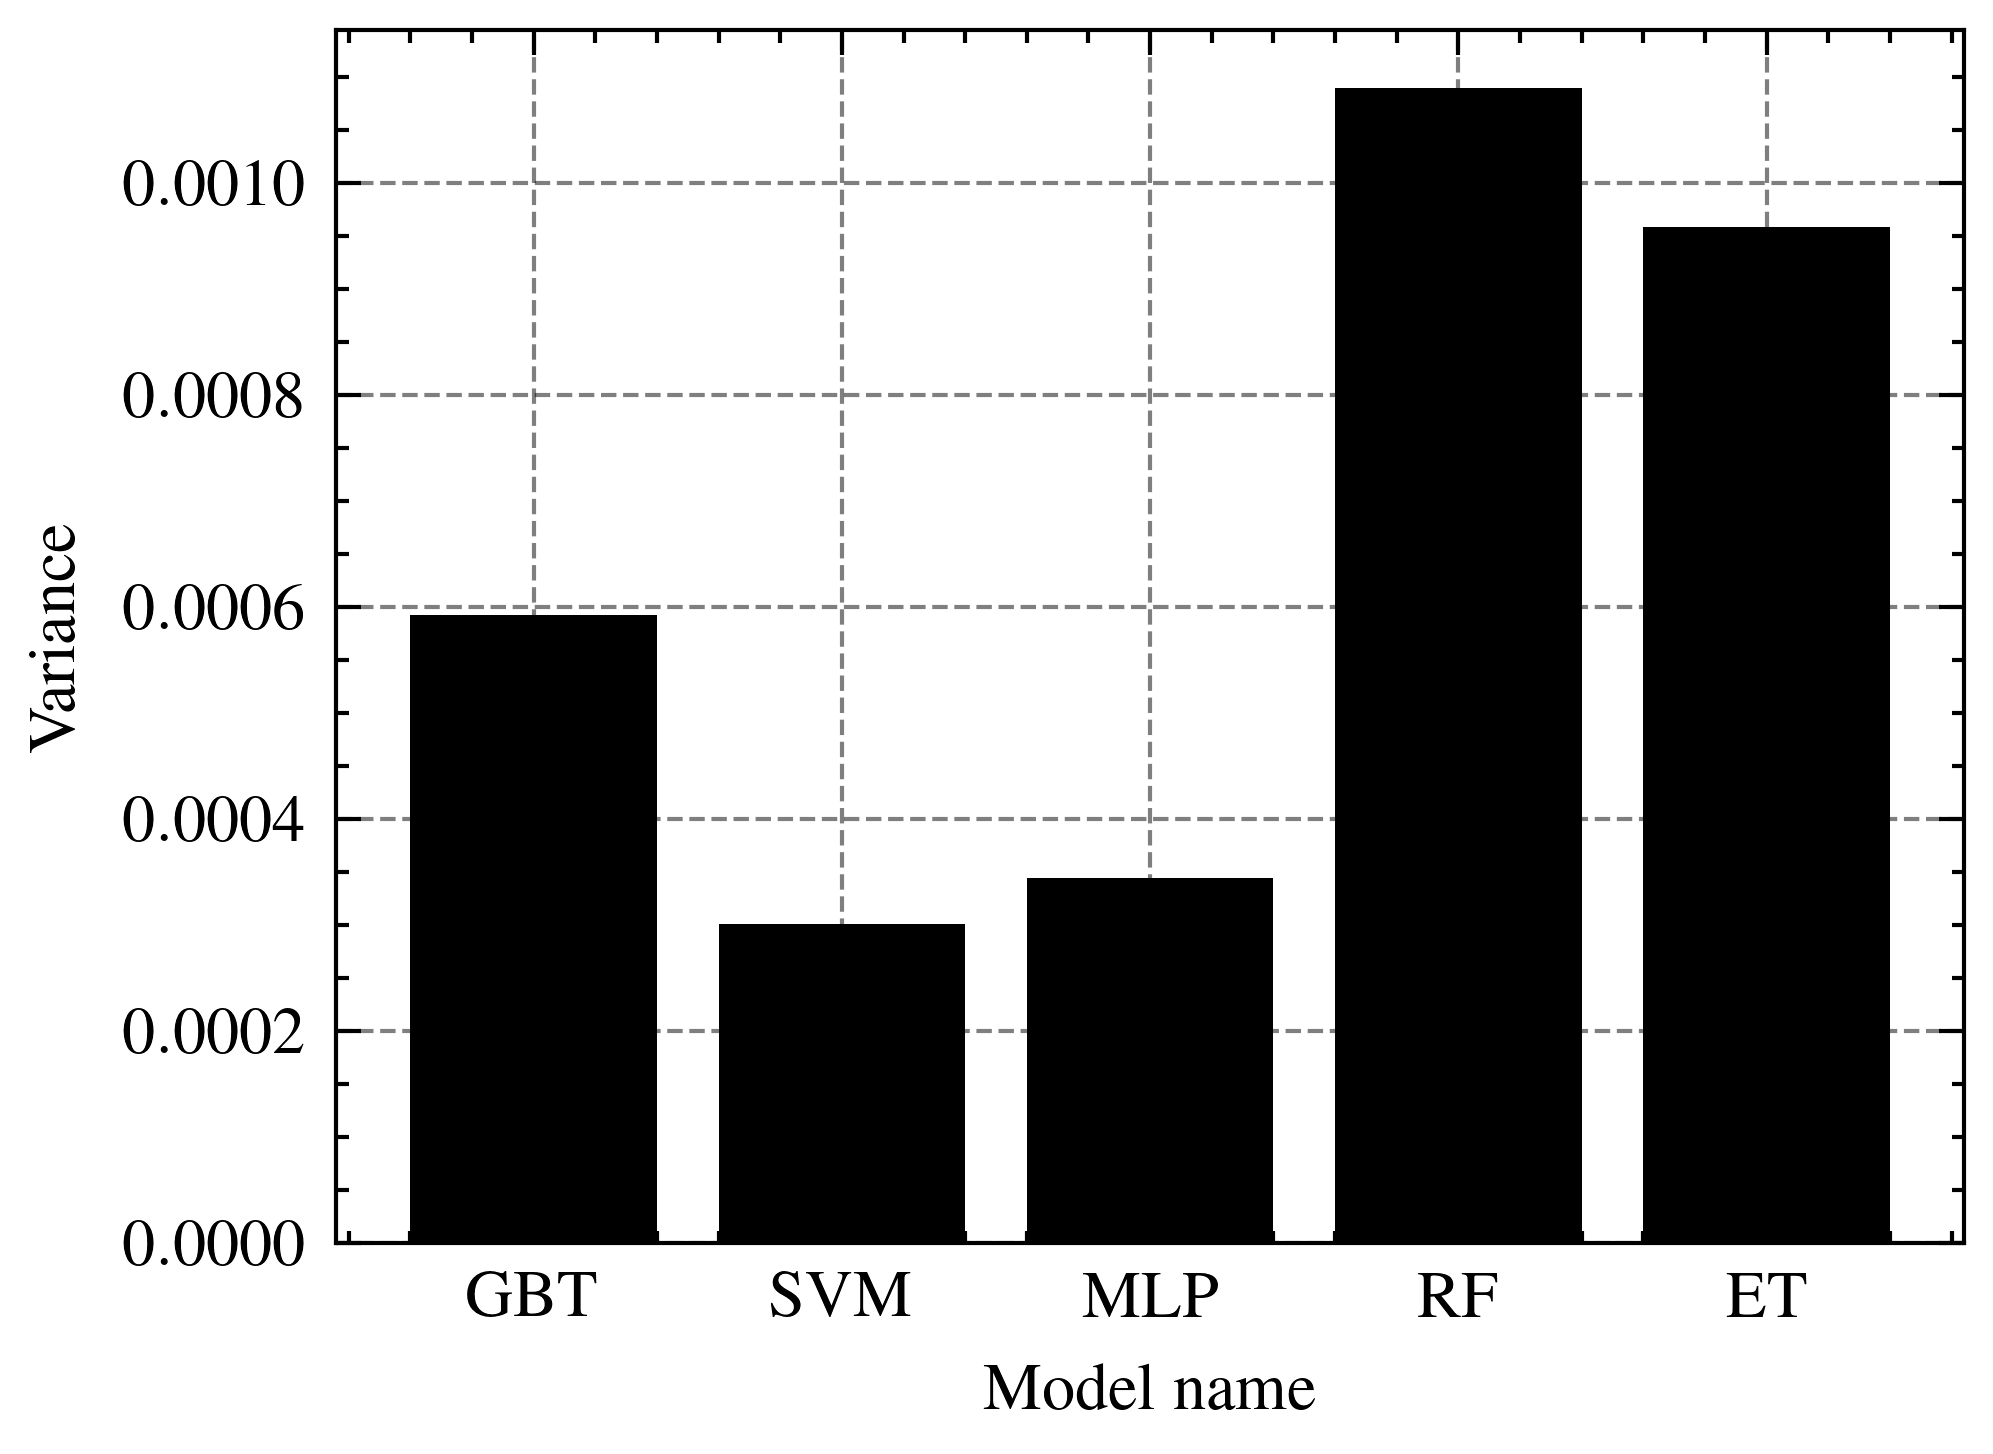
\includegraphics[width=0.6\textwidth]{chap5/images/variance_missing_values}
    \end{tcolorbox}
    \caption{Variance of models when trained on different data.}
    \label{fig:variance-missing-values}
\end{figure}

\subsection{Noise}\label{subsec:noise}
A common practise in \ac{ML} is to add noise to the training data to improve
the model's generalization abilities.
In this study Gaussian Noise will be added to the data set to evaluate the robustness
of the model.
The noise will be added to the training data only as the training data should be as correct as possible to get
comparable results.

To add the noise, \textit{numpy.random.normal} function was used, which generate random numbers with a Gaussian
distribution~\cite{scikit-learn}.
The mean and standard deviations of each feature were calculated based on the original data, and the function was
used to generate noisy values for each feature.

To study the model's reaction to increasing amounts of noise, the noise added
to the training data was gradually increased starting from 1\% to 50\%, which means that in the
last iteration contains as many noisy as `clean' samples.
The difference between all \ac{RMSE} between iterations was defined as loss.
The total loss was calculated by averaging the difference of these values as shown in Equation~\ref{eq:noise}.

\begin{tcolorbox}[arc=0pt,boxrule=0.5pt]
    \begin{equation}
        \text{Average Loss} = \frac{1}{N} \sum_{i=1}^{N} |\text{RMSE}i -
        \text{RMSE}{avg}|\label
        {eq:noise}
    \end{equation}
\end{tcolorbox}

\begin{itemize}
    \item \textit{Does the calculation of the loss make sense?}
\end{itemize}

\subsection{Results}\label{subsec:results-robustness}
\cref{fig:results-noise-fig} presents the performance of models as more noise is introduced to the training
dataset.
The noisy dataset comprised 1000 samples, and the x-axis indicates the percentage of the original data that
was augmented with noise.
The dashed lines correspond to the default performance of the models in the absence of noise.

The results indicate that the performance of all models deteriorates rapidly with the addition of noise.
Specifically, the first 20\% of the noisy data causes the most significant decline in model performance, after which the
performance plateaus at a poor level.
It is noteworthy that the Extra Trees model exhibits the most robust performance, outperforming the Gradient Boosted
Trees and Random Forest models, which also demonstrate similar levels of resilience.

The results are interesting since they demonstrate that the typically high-performing SVM and MLP models
exhibit underperformance under the current conditions.
Specifically, the MLP is a highly expressive model with many parameters, making it prone to overfitting.
In this case, the addition of noise is likely causing the model to overfit to the noise, leading to poor
generalization performance.
On the other hand, the SVM aims to find an optimal hyperplane to separate the data with maximum margin, which makes
it highly sensitive to outliers and noise, making it challenging to identify the appropriate hyperplane.

These results emphasize the significance of selecting robust models and pre-processing the data to minimize the
presence of outliers.
Moreover, the study reveals that even a small amount of noise (i.e., 10\%) can significantly impact the model's
performance.
The significance of using a high-quality dataset is emphasized.
Also, the results indicate that a smaller dataset can still be effective in model training as long as the data
quality is good.

\begin{figure}[h]
    \begin{tcolorbox}[arc=0pt,boxrule=0.5pt]
        \centering
        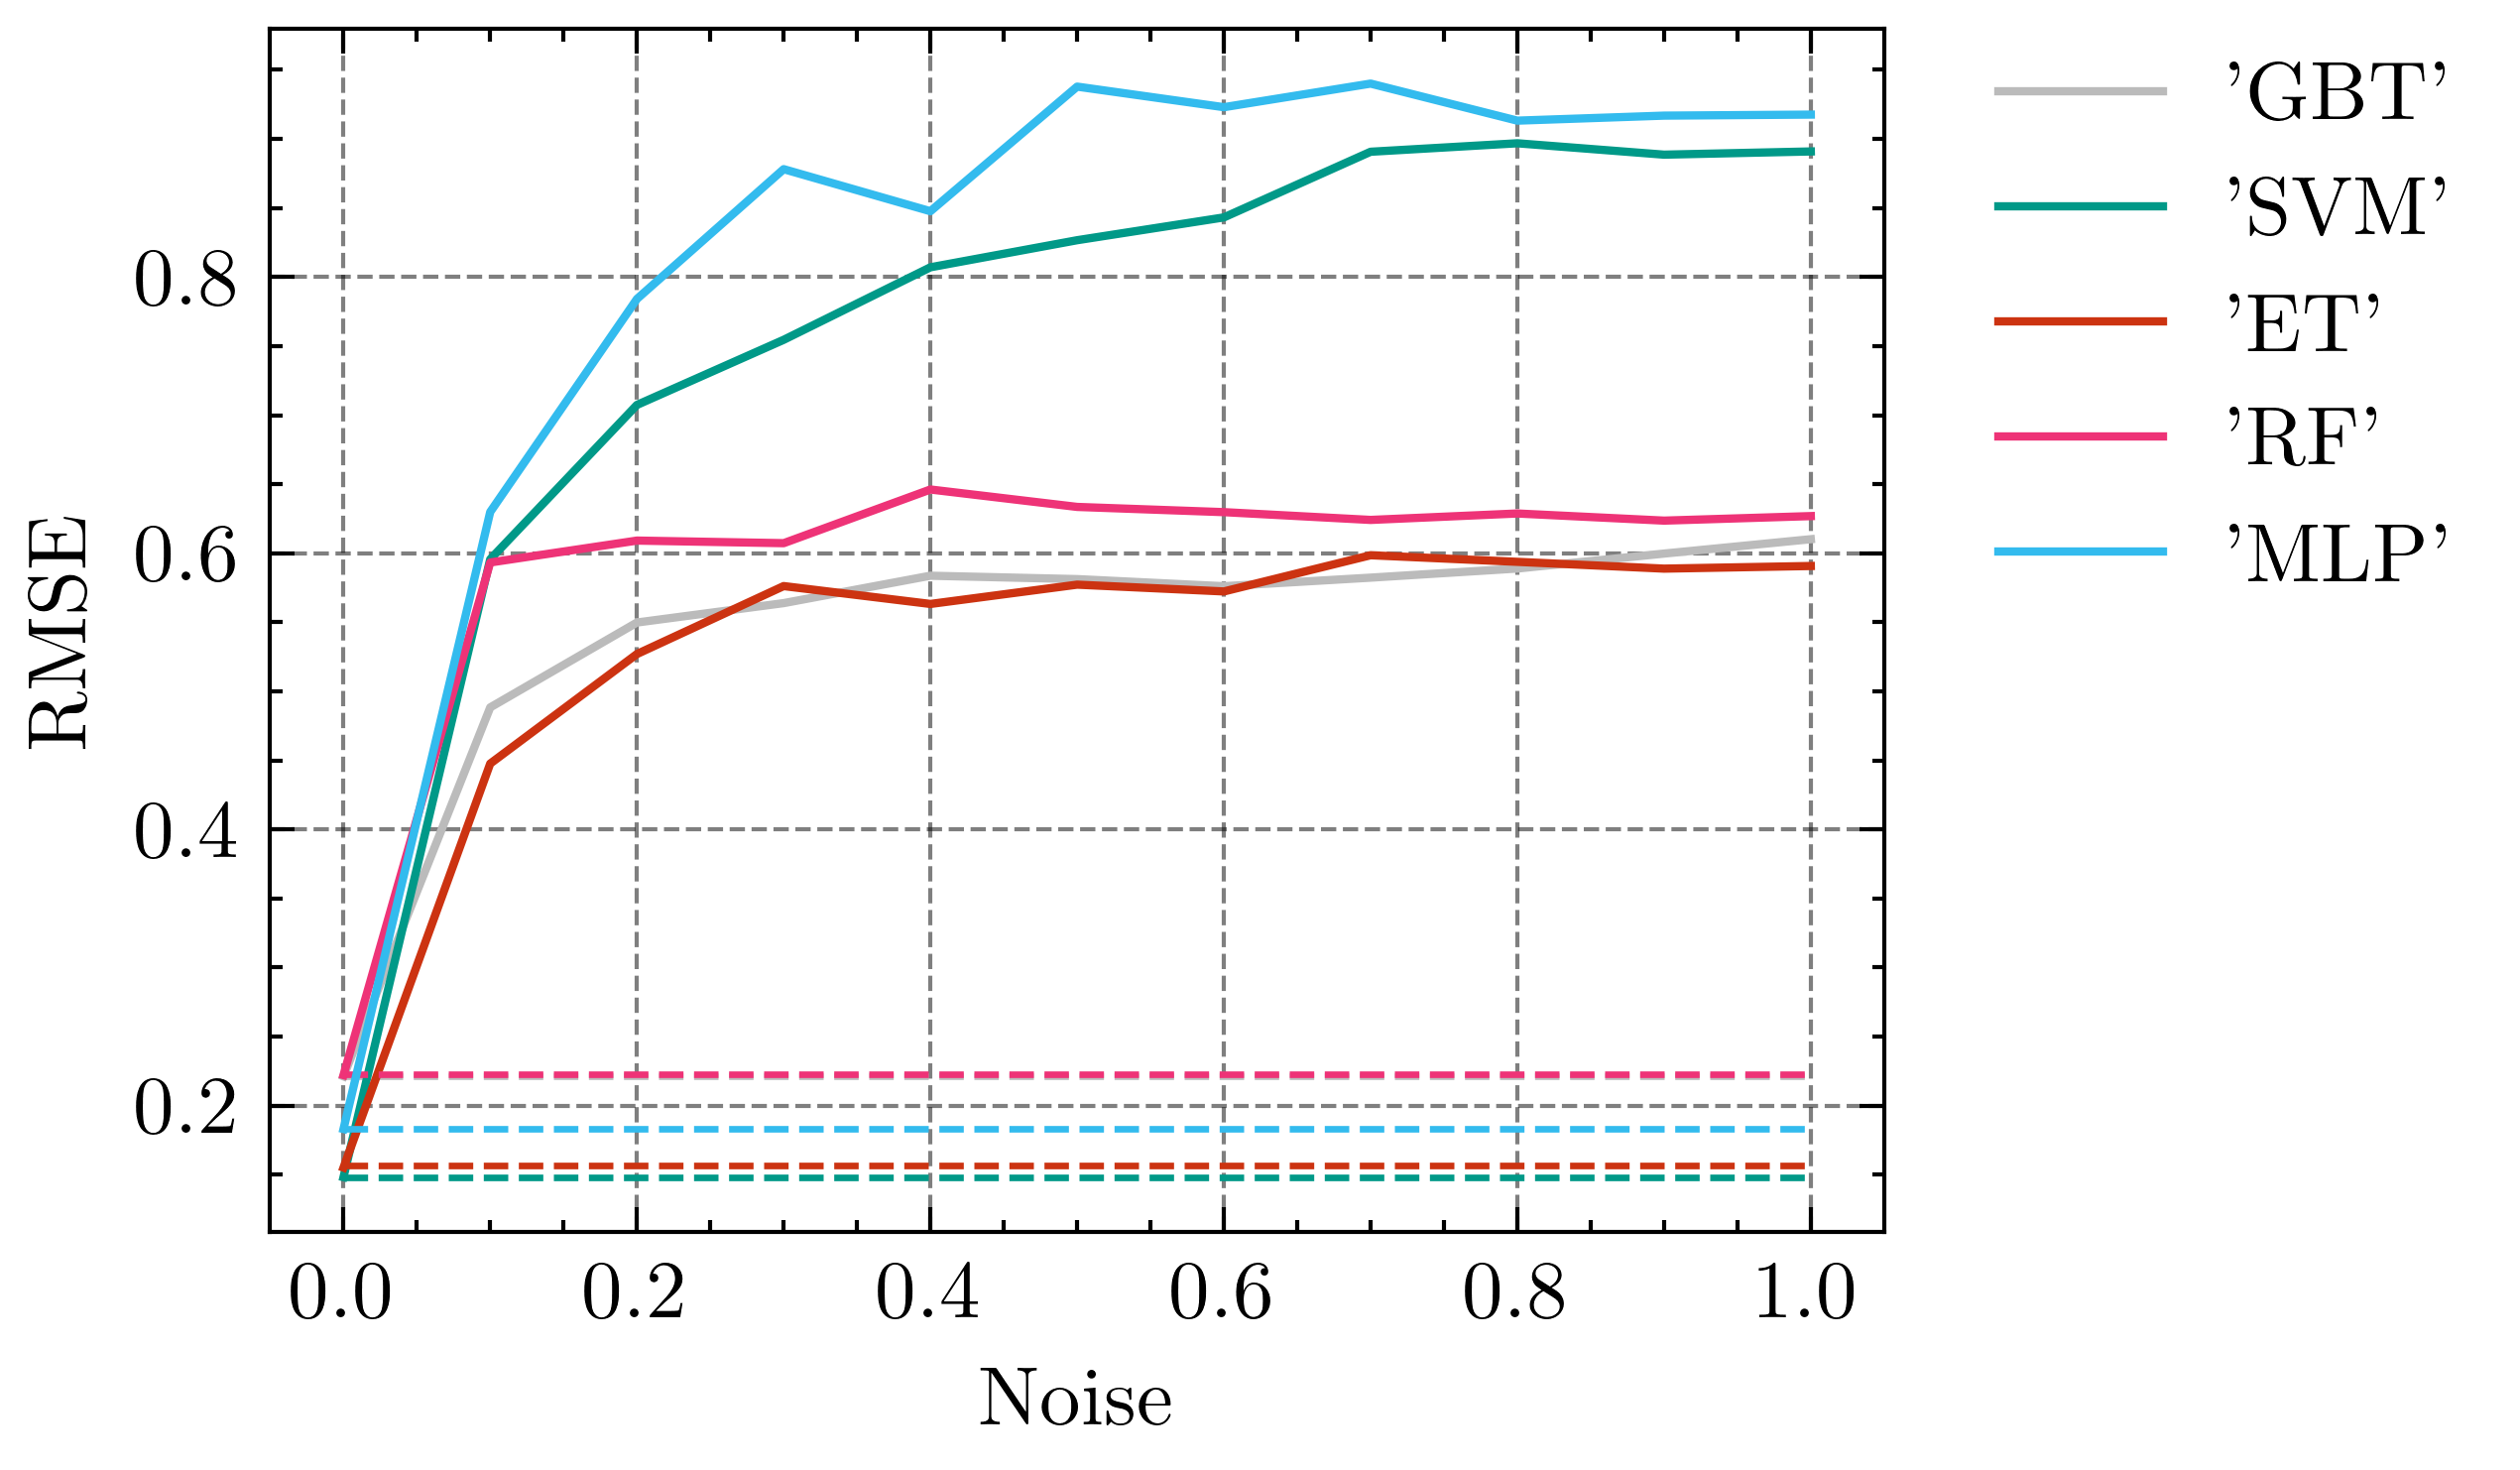
\includegraphics[width=0.9\textwidth]{chap5/images/results_noise}
    \end{tcolorbox}
    \caption{Comparison of performance on noisy data.
    The x-axis shows how many percent of the noisy dataset where added to the training data.
    The y-axis shows the MSE metric.
    The dotted lines show the default performance of the model.
    The solid lines show the performance of the model when noise was added to the training data.
    }
    \label{fig:results-noise-fig}
\end{figure}


\section{DP4: Stability}\label{sec:stability}
To evaluate the stability of the models, the Leave-One-Out Cross-Validation (LOOCV) can be used.
LOOCV, a type of Cross-Validation in which one sample is used for validation and the remaining data is used for
training, is one appropriate way to measure a model's stability.
~\cite[p. 200--201]{gareth2013introduction}.
To evaluate the model's stability, the \ac{LOOCV} was repeated for all samples in the dataset, resulting in a total
of $n$ iterations.
The stability of the model was then determined by calculating the average prediction error across all iterations,
using the equation provided in \cref{eq:loocv}~\cite[p. 201]{gareth2013introduction}.

\begin{tcolorbox}[arc=0pt,boxrule=0.5pt]
    \begin{equation}
        CV_{(n)} = \frac{1}{n} \sum_{i=1}^{n} \text{MSE}_{i}\label{eq:loocv}
    \end{equation}
\end{tcolorbox}

Usually the MSE is used as the error metric since it is not needed the RMSE is just the square root of the MSE and
therefore does not provide any additional information.
Additionally the resulting (\ac{MSE}) is a poor estimate of the model's
generalization error since only one sample is used for validation.
But the metric can be used to evaluate the model's stability, which is the goal of this section.
The final stability is determined by the standard deviation of the cross-validation scores
~\cite[p. 201]{gareth2013introduction}.
A low standard deviation across all folds indicates that the model can generate consistent results when trained on
different datasets, which suggests a more stable model.

It is worth mentioning that there are numerous methods for determining a model's stability.
In this study, \ac{LOOCV} was chosen for several reasons:
First, \ac{LOOCV} uses almost all the available data for training, while k-fold cross -validation reserves a portion
of the data for testing.
Since the dataset used in this study is relatively small, using all the data for training is advantageous.
Second, \ac{LOOCV} typically has lower bias due to the larger training set.
Lastly, various approaches were attempted to measure the model's stability, and \ac{LOOCV} delivered
the most stable and interpretable results.
The primary drawback of this method is its computational expense since it
requires $n$ iterations.

\cref{subsec:results-stability} presents the cross-validation score and standard deviation for each model.
The focus of the analysis is on the standard deviation since it provides a better indication of the model's stability.
As mentioned earlier, the \ac{CV} score using \ac{LOOCV} is a poor estimator of the model's generalization error.

\subsection{Results}\label{subsec:results-stability}

\cref{tab:results-stability} shows the mean cross-validation score and standard deviation for each model.
In order to evaluate the stability of the model, the standard deviation was used as the primary metric.
The stability analysis using LOOCV reveals that the Gradient Boosting model is the most stable with a standard
deviation of 0.183.
The Etra Trees and Random Forest model exhibit similar levels of stability with mean CV scores of 0.047 and 0.049,
and standard deviations of 0.206 and 0.194
It can be observed again, similar to the evaluation of the robustness that the MLP and SVM models exhibit
lower stability levels compared to the other models even though they where the most promising in the evaluation of
the correctness.

While stability is an important factor to consider, other aspects in particular the generalization error (correctness)
should be also taken into account.

\begin{table}[h]
    \begin{tcolorbox}[arc=0pt,boxrule=0.5pt]
% \sisetup{group-minimum-digits = 4}
        \centering
        \begin{tabular}{ll}
            \toprule
            \thead{\textbf{Model Name}} & \thead{\textbf{mean cv score ± std}}
            \\
            \toprule
            \textbf{Gradient Boosting}      & 0.038 ± 0.183 \\
            \hdashline
            \textbf{Random Forest}          & 0.047 ± 0.206 \\
            \hdashline
            \textbf{Extra Trees}            & 0.049 ± 0.194 \\
            \hdashline
            \textbf{Support Vector Machine} & 0.053 ± 0.244 \\
            \hdashline
            \textbf{MLP}                    & 0.053 ± 0.244 \\
            \hdashline
            \bottomrule
        \end{tabular}
    \end{tcolorbox}
    \caption{Results of the stability of the models.}
    \label{tab:results-stability}
\end{table}


\section{DP5: Resource utilization}\label{sec:resource-utilization}

To evaluate the resource utilization of the model, several metrics can be employed.
As discussed in \cref{subsec:dp5-resource-utilization}, this study focuses on time, computational power,
and memory resources.
Consequently, the metrics utilized to assess resource utilization include training time, inference time, and memory
usage.

The training time is measured in seconds and refers to the time that is required to train the model.
Training a model need computational resources such as memory and CPU power, thus the longer the training process
takes the more resources are needed.
Therefore a shorter training time is preferred.
To measure the training time the python function \texttt{time.time} is employed.
The functions does return the time in seconds since the epoch.
The time is recorded when the model is fitted and the difference between the two values
represents the training time.

The inference time is measured in milliseconds and refers to the time the models need to make predictions.
This metric is important for real-world use cases because user do not want to wait long for predictions and the
process also needs computational resources.
Since most models are able to make one predictions quite fast the inference time is measured for 100 predictions
using the \texttt{time.time} function again.

The memory usage is measured in megabytes (MB) and refers to the amount of memory that is required to run and save
the mode.
A smaller memory footprint is preferred because it required less resources in the form of storage space.
To measure the memory usage the \texttt{memory\_usage} function from the package \texttt{memory\_profiler} is
employed.


\subsection*{Results}

\cref{tab:results_resource_utilization} shows the results for the text that where made.
Looking at the training time the Extra Trees and Random Forest model perform the with the shortest training times
of 19.541 and 24.912 ms
The Support Vector Machine and Gradient boosted model have intermediate training times.
The MLP is clearly the slowest with over 16 seconds.
The training time can be attributed the nature of the models and their training algorithm.
The RF and ET both benefit from the bagging technique which means that they training an ensemble of decision trees and
combine them to one big model.
This can be done in parallel and therefore massively speeds up the training
process (see \ref{subsubsec:random-forests}).
On the other side MLPs are typically more computational since feeding forward and backpropagation are not
parallelize and computationally expensive in general (see \cref{subsec:neural-networks}).

A comparable picture can be derived for the inference time.
This time the GBR, which is also a tree based algorithm is the fasted to make predictions while the MLP is the slowest.
The ET, RF and SVM models have comparable times.

Looking at the memory usage the models are quite similar with the MLP using the most memory 170 KB.
The other models have quite similar memory usage ranging from 157 to 158 KB.
Overall the memory space seems not to be a big issue for the models, a reason for that is the fact that the
dataset is not very big and the resulting models are also less complex.


\begin{table}[h]
    \begin{tcolorbox}[arc=0pt,boxrule=0.5pt]
        \centering
        \begin{tabular}{llll}
            \toprule
            \thead{\textbf{Model Name}} & {\thead{\textbf{Training time} \\
            \unit[]{ms}}}
            & {\thead{\textbf{Inference time} \\ \unit[]{ms}}} &
                {\thead{\textbf{Memory Usage} \\
            \unit{kb}}}
            \\
            \toprule
            \textbf{ET}  & 19.541     & 1.939  & 157.93 \\
            \hdashline
            \textbf{RF} & 24.912     & 2.027  & 157.684 \\
            \hdashline
            \textbf{GBR} & 43.688    & 1.302  & 158.121 \\
            \hdashline
            \textbf{SVM} & 421.007 & 2.587 & 158.082 \\
            \hdashline
            \textbf{MLP} & 16466.261s & 17.988 & 170.715 \\
            \bottomrule
        \end{tabular}
    \end{tcolorbox}
    \caption{Overview of the used machine learning models and their metrics.}
    \label{tab:results_resource_utilization}
\end{table}


\section{DP6: Interpretability}\label{sec:interpretability}
In accordance with the definitions of interpretability outlined in \cref{sec:objectives-of-a-solution}, it
becomes apparent that quantitatively measuring interpretability is not viable.
However, alternative approaches can be employed to gauge a model's interpretability.

%\cite{molnar2020interpretable} distinguishes between model-specific and model-agnostic approaches.
%Model-specific procedures are particular to one model, but model-agnostic methods can be applied to any model.
%~\cite[p. 19]{molnar2020interpretable}.

One strategy for achieving interpretability is restricting the selection of algorithms to those that yield
model specific interpretable outcomes.
Interpretable algorithms used in this study are Linear Regression and Decision
Trees~\cite[p. 35]{molnar2020interpretable}.
Nonetheless, as discussed in \cref{sec:dp1:-correctness}, these algorithms do not demonstrate sufficient
performance to be deemed viable solutions for predicting spring back.
Consequently, this study cannot rely on model-specific interpretability methods and should instead utilize model
-agnostic methods for generating explanations.

Also~\cite{doshi2017towards} differentiates between global and local interpretability.
Global interpretability refers to the ability to understand the overall behavior of
the model, while local interpretability refers to the ability to understand the behavior of the
model for a specific instance.
It does not make sense to apply model-agnostic method on all trained models, it makes more sense to
apply the methods on the best performing models.
% TODO and Extra Trees...
In the other parts of the evaluation, the Random Forest, Support Vector Machine and Multi Layer Perceptron models
where always under the best perfoming models and are therefore the models that are used in the following
sections.

\subsection{Global Model-Agnostic Methods}\label{subsec:global-model-agnostic-methods}
In the following section, global model-agnostic methods are applied to the trained machine learning models to
understand their overall behavior.

% TODO Source?
Two commonly used methods for analyzing the relationship between input features
and the target variable are Feature Dependence plots and Partial Dependence plots.
Feature dependence plots illustrate the relationship between a feature and the target variable.
By analyzing these plots, we can identify which features have the strongest impact on the model's
predictions, making it easier to prioritize and refine our feature selection.

In the case of \ac{MLP}, there is no built-in feature importance, as the importance of each feature is determined by
the weights assigned to the perceptron.
For \ac{SVM}, feature importance cannot be directly derived from the model
because the algorithm applies a hyperplane that separates the data.
The importance of a feature depends on the influence of the hyperplane, which is not easily measurable.
Consequently, feature importance cannot be plotted for
the two chosen models.
In contrast, other models, such as random forests, have built-in feature importance that can
be utilized to analyze the model.


\ref{fig:feature-importances-rf1} compares and visualizes the relative importance of the features used for
training the model.
The figure was created using the \texttt{feature\_importances\_} attribute of the \texttt{RandomForestRegressor}
model from the \texttt{scikit-learn} library.
The Partial Dependence Plots (PDP) provide insights into the relevance and interactions of the
features.
As illustrated, thickness is the most important feature, followed by distance and die opening.
This means that changes in thickness have the most significant impact on spring back, while variations in the other two features
have a comparatively smaller influence on the outcome.
In terms of interactions, all features are relevant, indicating that each feature contributes unique information to
the model.
This could suggest that the features are not highly correlated with each other, as their interactions
could already be observed in the correlation matrix shown in Figure~\ref{fig:correlation_matrix}.
Consequently, removing one feature would result in a significant loss of information and, therefore, poorer
performance of the model.

\begin{figure}[h]
    \begin{tcolorbox}[arc=0pt,boxrule=0.5pt]
        \centering
        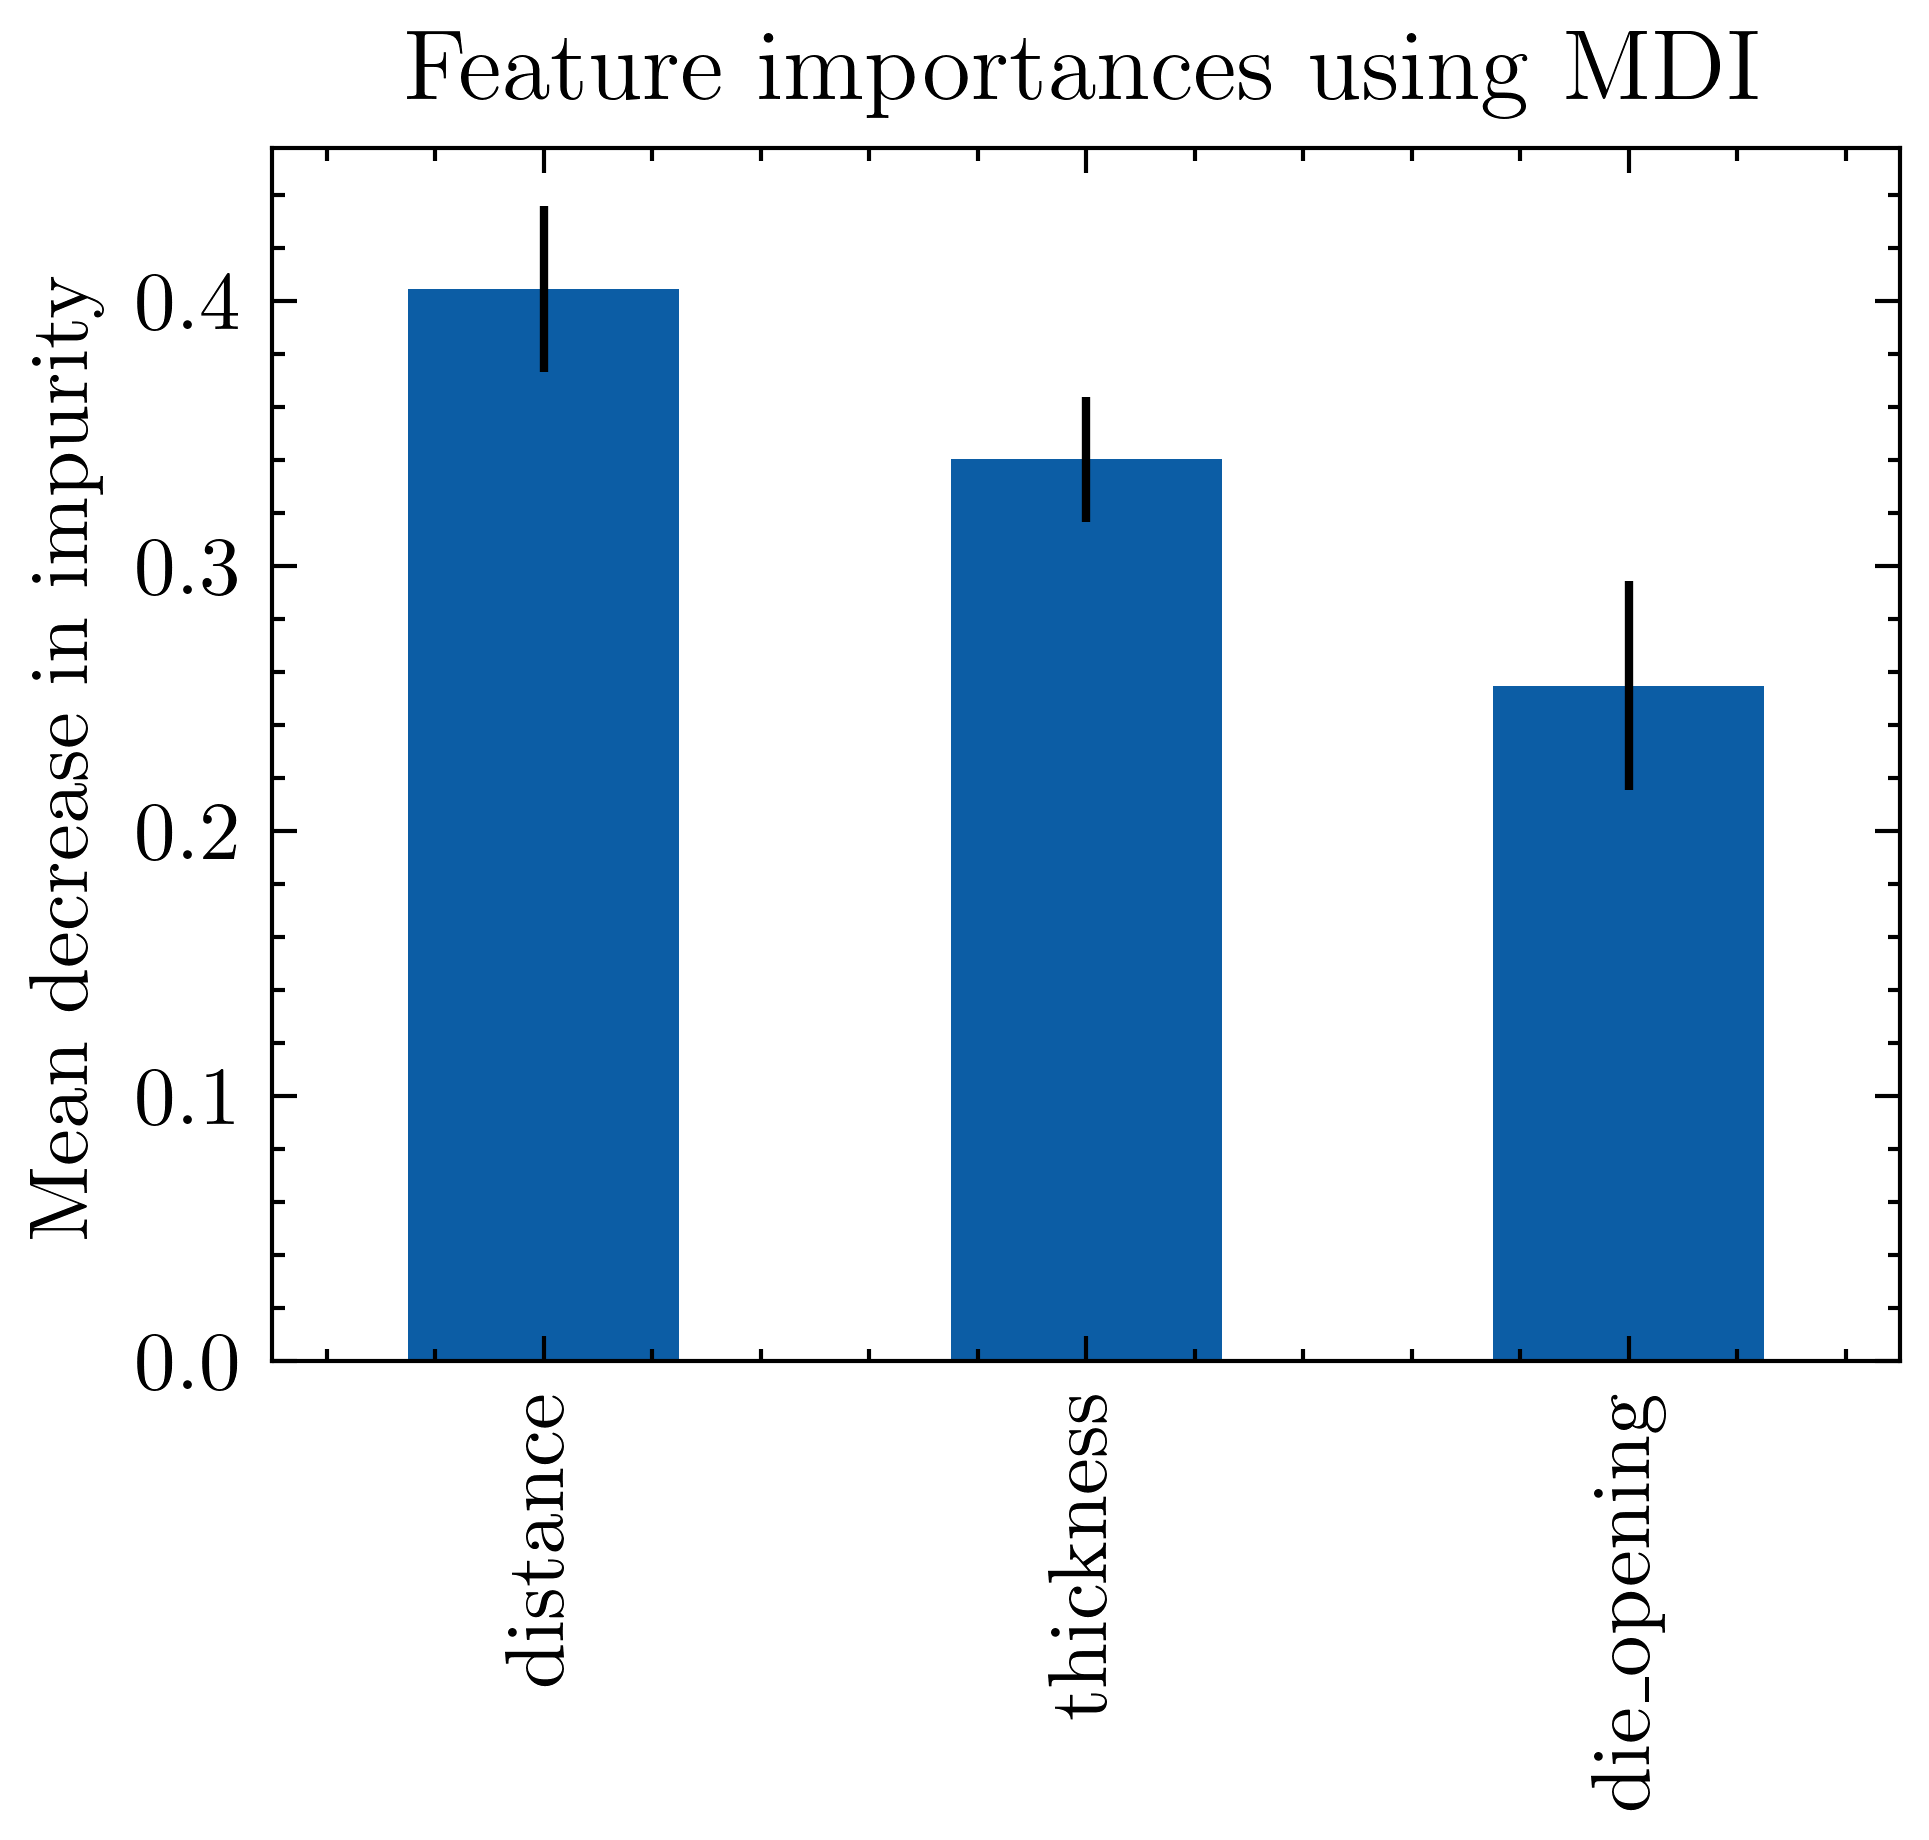
\includegraphics[width=0.7\textwidth]{chap5/images/rf_feature_importances}
    \end{tcolorbox}
    \caption{Feature importance of the random forest model.}
    \label{fig:feature-importances-rf1}
\end{figure}

The feature importance plot did facilitate a better understanding of the relationship between the features and the
target
variable.
However, they do not provide insights into exactly how the features influence the outcome. Partial dependence plots
can be helpful for this purpose.

\subsubsection{Partial Dependence}
\cite{greenwell2018simple} introduced another feature importance measure based on partial dependence.
Partial dependence refers to the relationship between a target variable and a single predictor variable in a statistical
model, while keeping all other predictor variables constant.
A feature that exhibits a consistent partial dependence across all values is less important than a feature that

Partial dependence plots examine the impact of a single input feature on the target variable while keeping all other
features constant.
While the feature importance plot shows the relative importance of each feature, the partial dependence plot shows
the impact of a single feature on the target variable.

In Figure~\ref{fig:partial_dependence_plots}, we can see the PDPs for two models: Support Vector Machines (SVM) and
Multilayer Perceptron (MLP).
It can be seen that the plots for both models yield the same results for the three features.
The results show that a higher $y_p$ value leads to a greater spring back, while
increasing the thickness of the metal sheet results in a lower spring back.
The effect of the die opening is less
significant than the other two features, but there is still a noticeable increase in spring back with higher die
opening.
The PDPs demonstrate that all features exhibit a non-linear relationship with the target variable.
This information can be useful for understanding the behavior of the models and the impact of different features on
the predicted outcome.

\begin{figure}[h]
    \begin{tcolorbox}[arc=0pt,boxrule=0.5pt]
        \centering
        \begin{subfigure}{0.45\textwidth}
            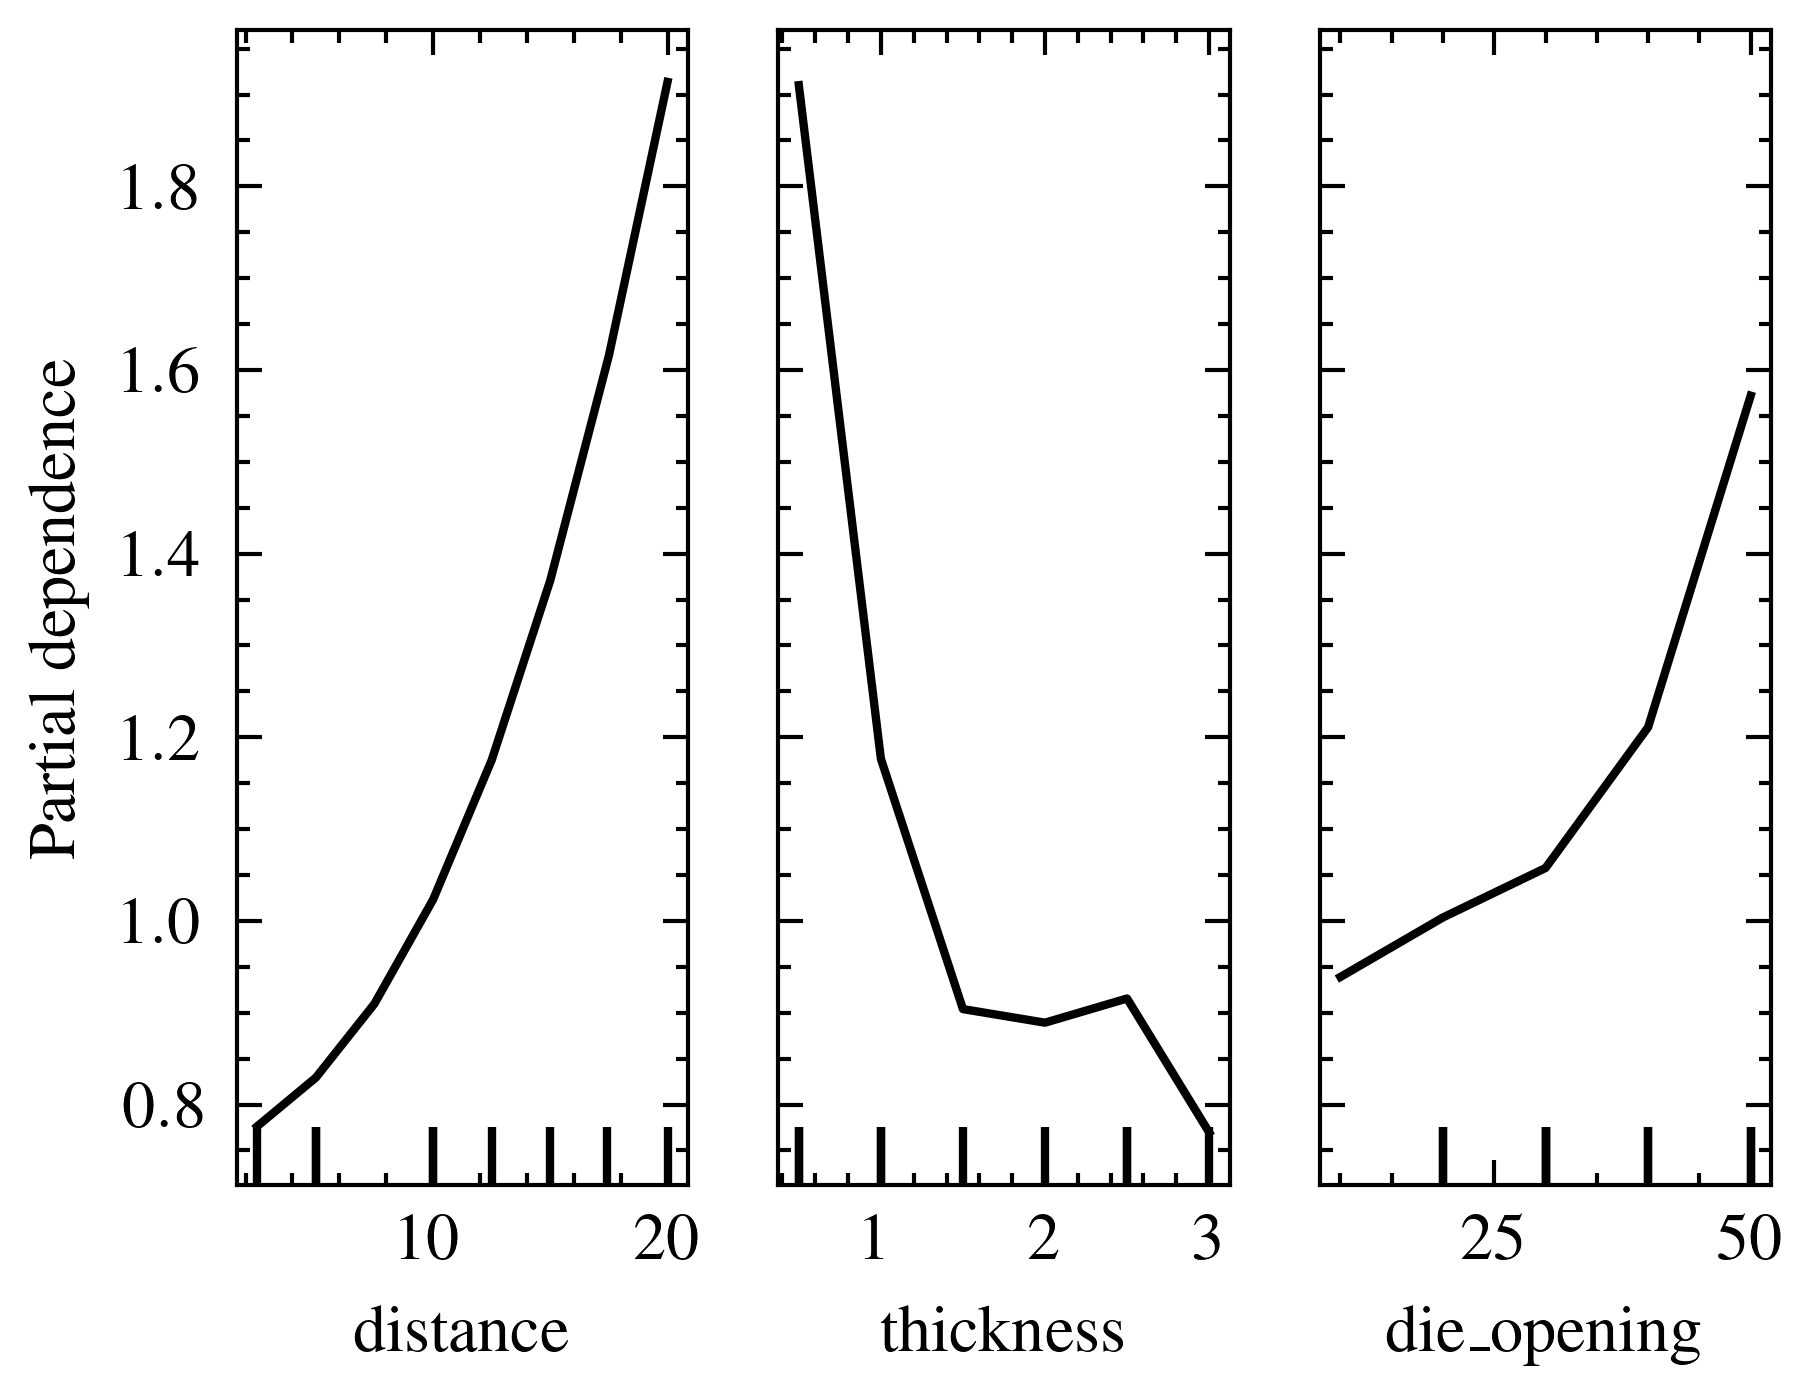
\includegraphics[width=\textwidth]{chap5/images/partial_dependence_SVM}
            \caption{SVM}
            \label{fig:feature_impoartances_rf}
        \end{subfigure}
        \hfill
        \begin{subfigure}{0.45\textwidth}
            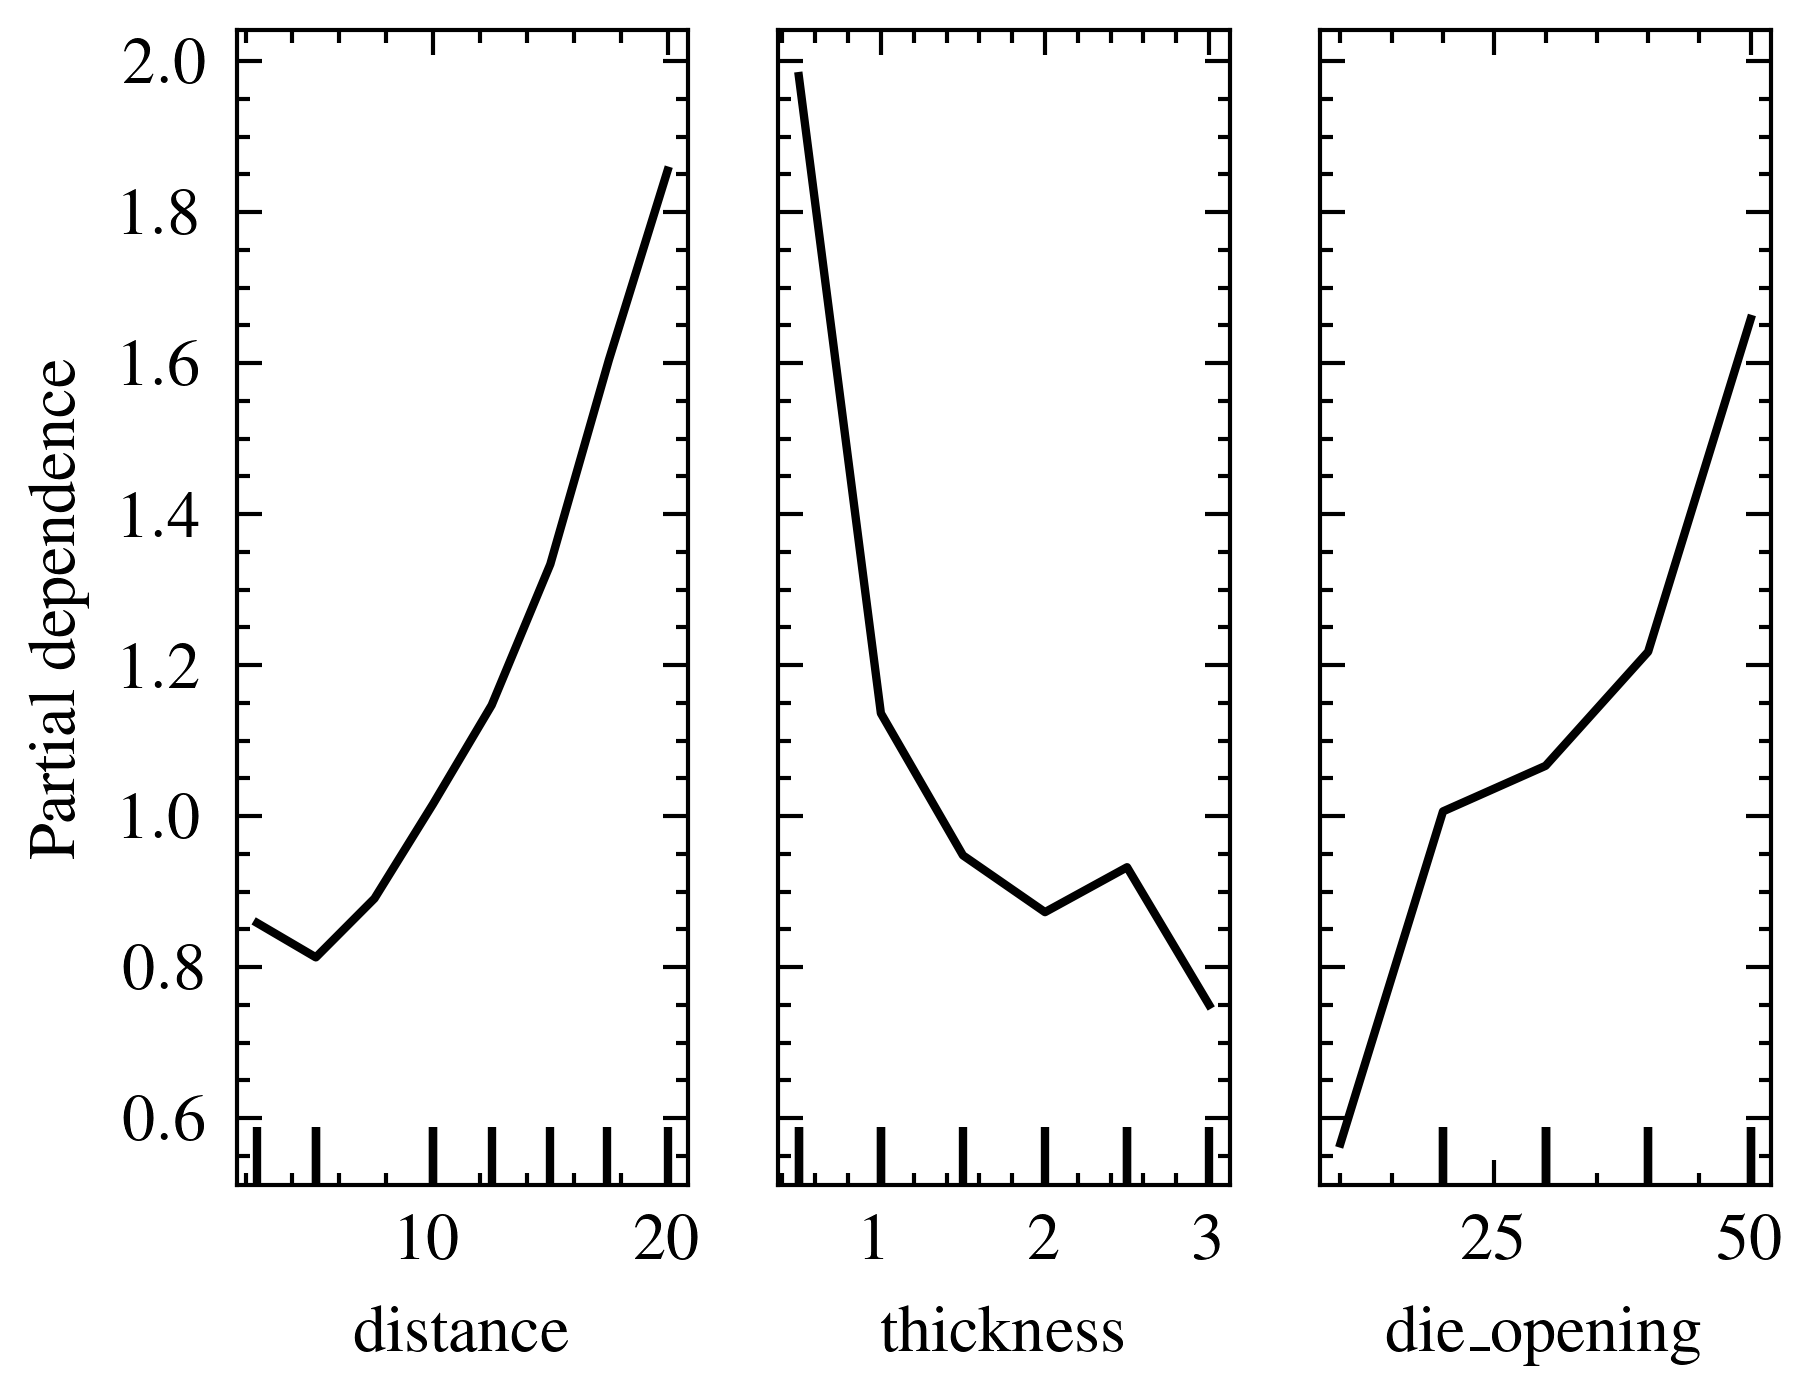
\includegraphics[width=\textwidth]{chap5/images/partial_dependence_MLP}
            \caption{MLP}
            \label{fig:partial_dependence_svm}
        \end{subfigure}
        \hfill
    \end{tcolorbox}
    \caption{Partial dependence plots}
    \label{fig:partial_dependence_plots}
\end{figure}

It is important to note that partial dependence plots and feature importance plots are limited to
identifying linear relationships between features and the target variable.
Since this is not the case as state previously, the results of the partial dependence plots are
alternative models as permutation feature importance and SHAP values are used to gain further
information.

\subsection{Permutation Feature Importance and SHAP}\label{subsec:permutation-feature-importance-
and-shap}

Permutation feature importance's assesses the impact on the model's prediction error when the values
of a feature a randomly permutes.
Permutation in this context means the process of randomly shuffling the values of a single features while keeping the
values of all other feautres unchanged.
Thereby the association between the feature and the actual outcome is disrupted~\cite[p. 157]{molnar2020interpretable}.

The importance of a feature is evaluated by assessing the degree to which permuting its values
results in an increase in the prediction error fo the model.
If permuting a features results in a significant increases in errors the features is deemed
important because the model relied on it for making accurate predictions.
Conversely, if permuting a feature doesn't change the prediction error is considered unimportant
because the model didn't utilize it for its prediction~\cite[p. 158]{molnar2020interpretable}.

The resutls presented in Figure~\ref{fig:permutation_feature_importance} show that hte MLP and the SVM models yield
similar trends in the importance of features.
The feautres thickness and punch penetrration have a high importance with their permutation causing a significant
increase
in the prediction error both in $R^2$ and $MSE$.
This inidicates that they are crucial for the decision making of the model.

Different from the previous plots, the die opening has a importance of zero in both models.
Ths implies does permuting this features does not have any influence on the prediction error.
There are two possible explanations for this.

1. The die opening is not relevant for the decision making and does not provide any significant information.

2. The die opening is important but only in combination with either the thickness or the penetration distance.
This suggest that there might be an interactions effect that was not captures in previous analysis.

Since the normal feature importance plots showed that die opening is important the second explanation is more likely.
To further investigate this possiblitly a partial dependence plot was created for the die opening in combination with
either the thickness or the penetration distance.

\begin{table}[h]
    \begin{tcolorbox}[arc=0pt,boxrule=0.5pt]
        \centering
        \subfloat[Subtable 1 list of tables text][MLP]{
            \begin{tabular}{lll}
                \toprule
                \multicolumn{3}{}{\textbf{$R^2$}} \\
                \toprule
                thickness   & 1.337 & +/- 0.173542 \\
                \hdashline
                distance    & 1.293 & +/- 0.145488 \\
                \hdashline
                die opening & 0.000 & +/- 0.000000 \\
                \toprule
                \multicolumn{3}{l}{\textbf{$MSE$}} \\
                \toprule
                thickness   & 0.274 & +/- 0.035613 \\
                \hdashline
                distance    & 0.265 & +/- 0.029856 \\
                \hdashline
                die opening & 0.000 & +/- 0.000000 \\
                \bottomline
            \end{tabular}}
        \qquad
        \subfloat[Subtable 2 list of tables text][SVM]{
            \begin{tabular}{lll}
                \toprule
                \multicolumn{3}{}{\textbf{$R^2$}} \\
                \toprule
                distance    & 1.237 & +/- 0.139285 \\
                \hdashline
                thickness   & 1.178 & +/- 0.157247 \\
                \hdashline
                die opening & 0.000 & +/- 0.000000 \\
                \toprule
                \multicolumn{3}{l}{\textbf{$MSE$}} \\
                \toprule
                distance    & 0.254 & +/- 0.028583 \\
                \hdashline
                thickness   & 0.242 & +/- 0.032269 \\
                \hdashline
                die opening & 0.000 & +/- 0.000000 \\
                \bottomline
            \end{tabular}}
    \end{tcolorbox}
    \caption{Permutation feature importance}
    \label{tab:permutation_feature_importance}
\end{table}

To investigate the joint performance of the die opening feature with the other two features,
again partial dependence plots can be used.
Figure~\ref{fig:partial_dependence_plots} shows a two-way partial dependence plot for the
\ac{MLP} model.
The x- and y-axes represent the thickness and the distance, respectively.
The slope of the contour lines indicates the direction of the effect of the die opening on the
prediction.
The contour lines are colored and labeled according to the value of the prediction.
It can be seen that the contour lines are not parallel which suggest the two features are
interaction with each other and therefore have a joint effect on the model prediction.
This means that the second explanation mentioned above is correct and the die opening is not irrelevant for the model
prediction but just interacts with the other two features.

\begin{figure}[h]
    \begin{tcolorbox}[arc=0pt,boxrule=0.5pt]
        \centering
        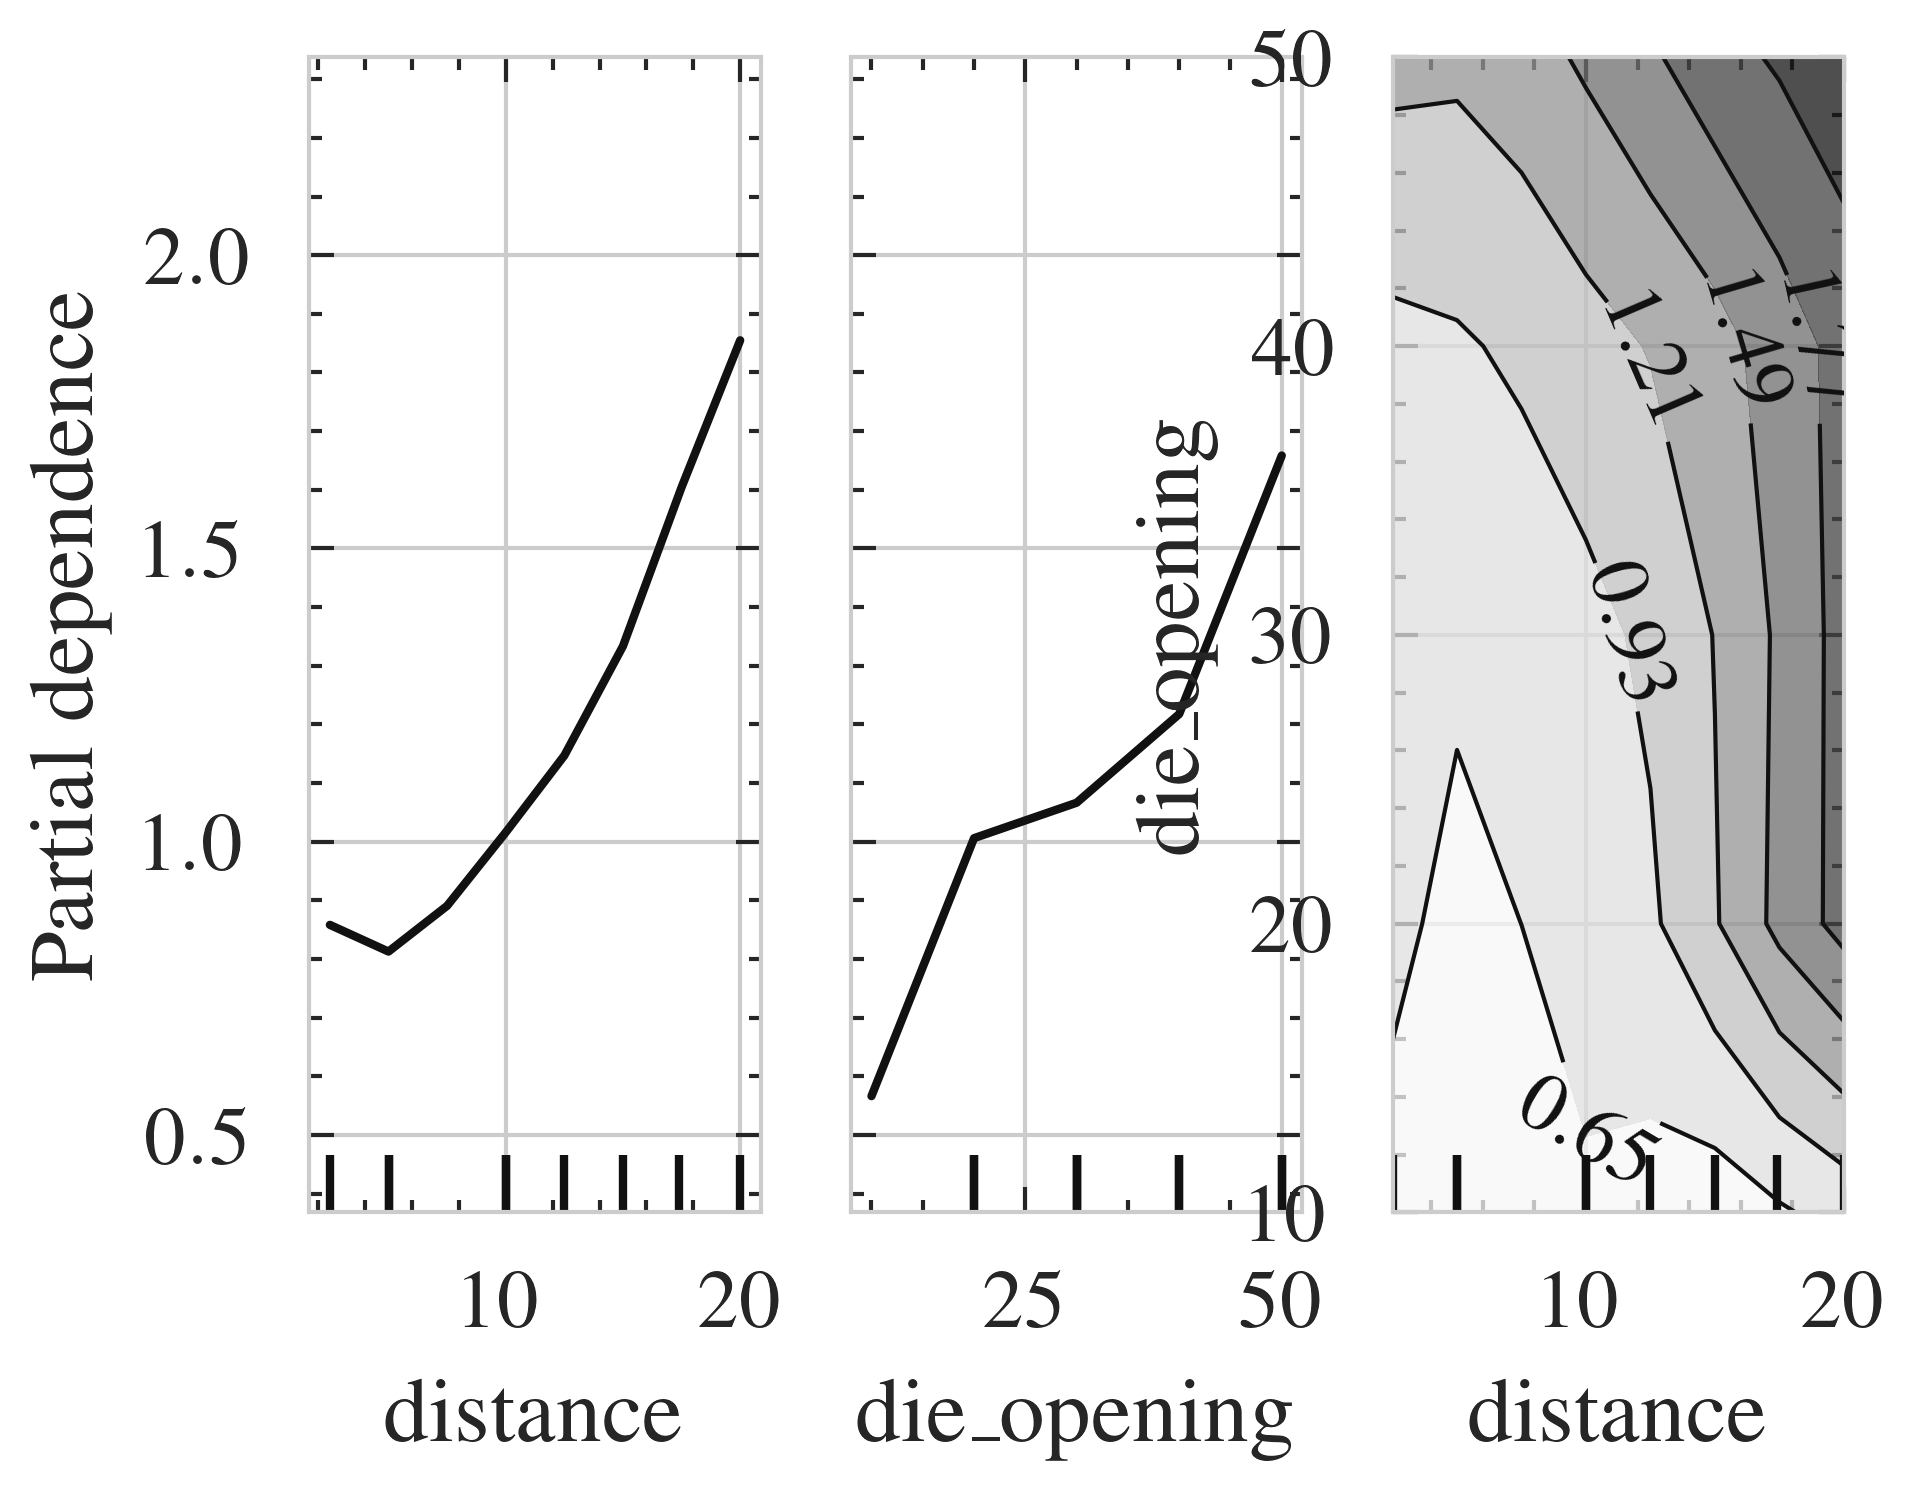
\includegraphics[width=0.8\textwidth]{chap5/images/pdp_distance_die_opening}
    \end{tcolorbox}
    \caption{DPD distance and die opening}
    \label{fig:dpd-distance-die-opening}
\end{figure}

\subsection{Local Model Agnostic Methods}\label{subsec:local-model-agnostic-methods}
Local interpretability refers to the ability to understand the behavior of the model for a
specific instance and is often used to explain the predictions of a model.
Model agnostic methods can be used to explain the predictions of any model type~\cite{molnar2020interpretable}.

Local methods rely on interpreting individual instances from a dataset, and as such, it is
crucial to select representative samples.
One way to achieve this is by considering the V/t ratio of each instance.

The local model agnostic method LIME was applied on different machine learning models.
But it did not yield any meaningful results.


\section{Demonstration}\label{sec:demonstration}
This section represents the demonstration activity in the \ac{DSR} process.
This activity focuses on the demonstration of the developed models in specific selected scenarios and not the
overall performance like in the evaluation activity.
For this purpose three scenarios are selected and the models are demonstrated in these scenarios.

For the current dataset, the V/t ratios range from 10 to 100.
The highest ratio can be achieved by bending a 0.5 mm thin metal sheet using a 50 mm wide die opening, while the
lowest ratio is achieved by bending a 1 mm thick sheet on a 10 mm die opening.

Recommended V/t ratios in industrial practices are between 6 and 10~\cite[p.7]{cruz_applicationmachinelearning_2021}.
Bending operations performed outside of this range of recommended ratios may result in
high spring back.
The lowest V/t ration in the dataset is 10, after that it was not possible to squeeze metals larger than 1 mm
through a die opening of 10 mm.
This means that the ratios used in industrial practise do not exactly apply of the dataset used in this study.

Upon examining Figure~\ref{fig:springback-heatmap}, it is evident that the V/t ratio has a significant impact on
spring back.
There appears to be a correlation between a greater die opening and a reduced thickness resulting in greater spring
backs.
Notably, the data points for $t0.5 V40$ and $t0.5 V50$ exhibit particularly elevated spring backs relative to the
remaining data set.
Conversely, all the data collected with a 10 mm die opening indicate lower spring back values.

\begin{figure}[h]
    \begin{tcolorbox}[arc=0pt,boxrule=0.5pt]
        \centering
        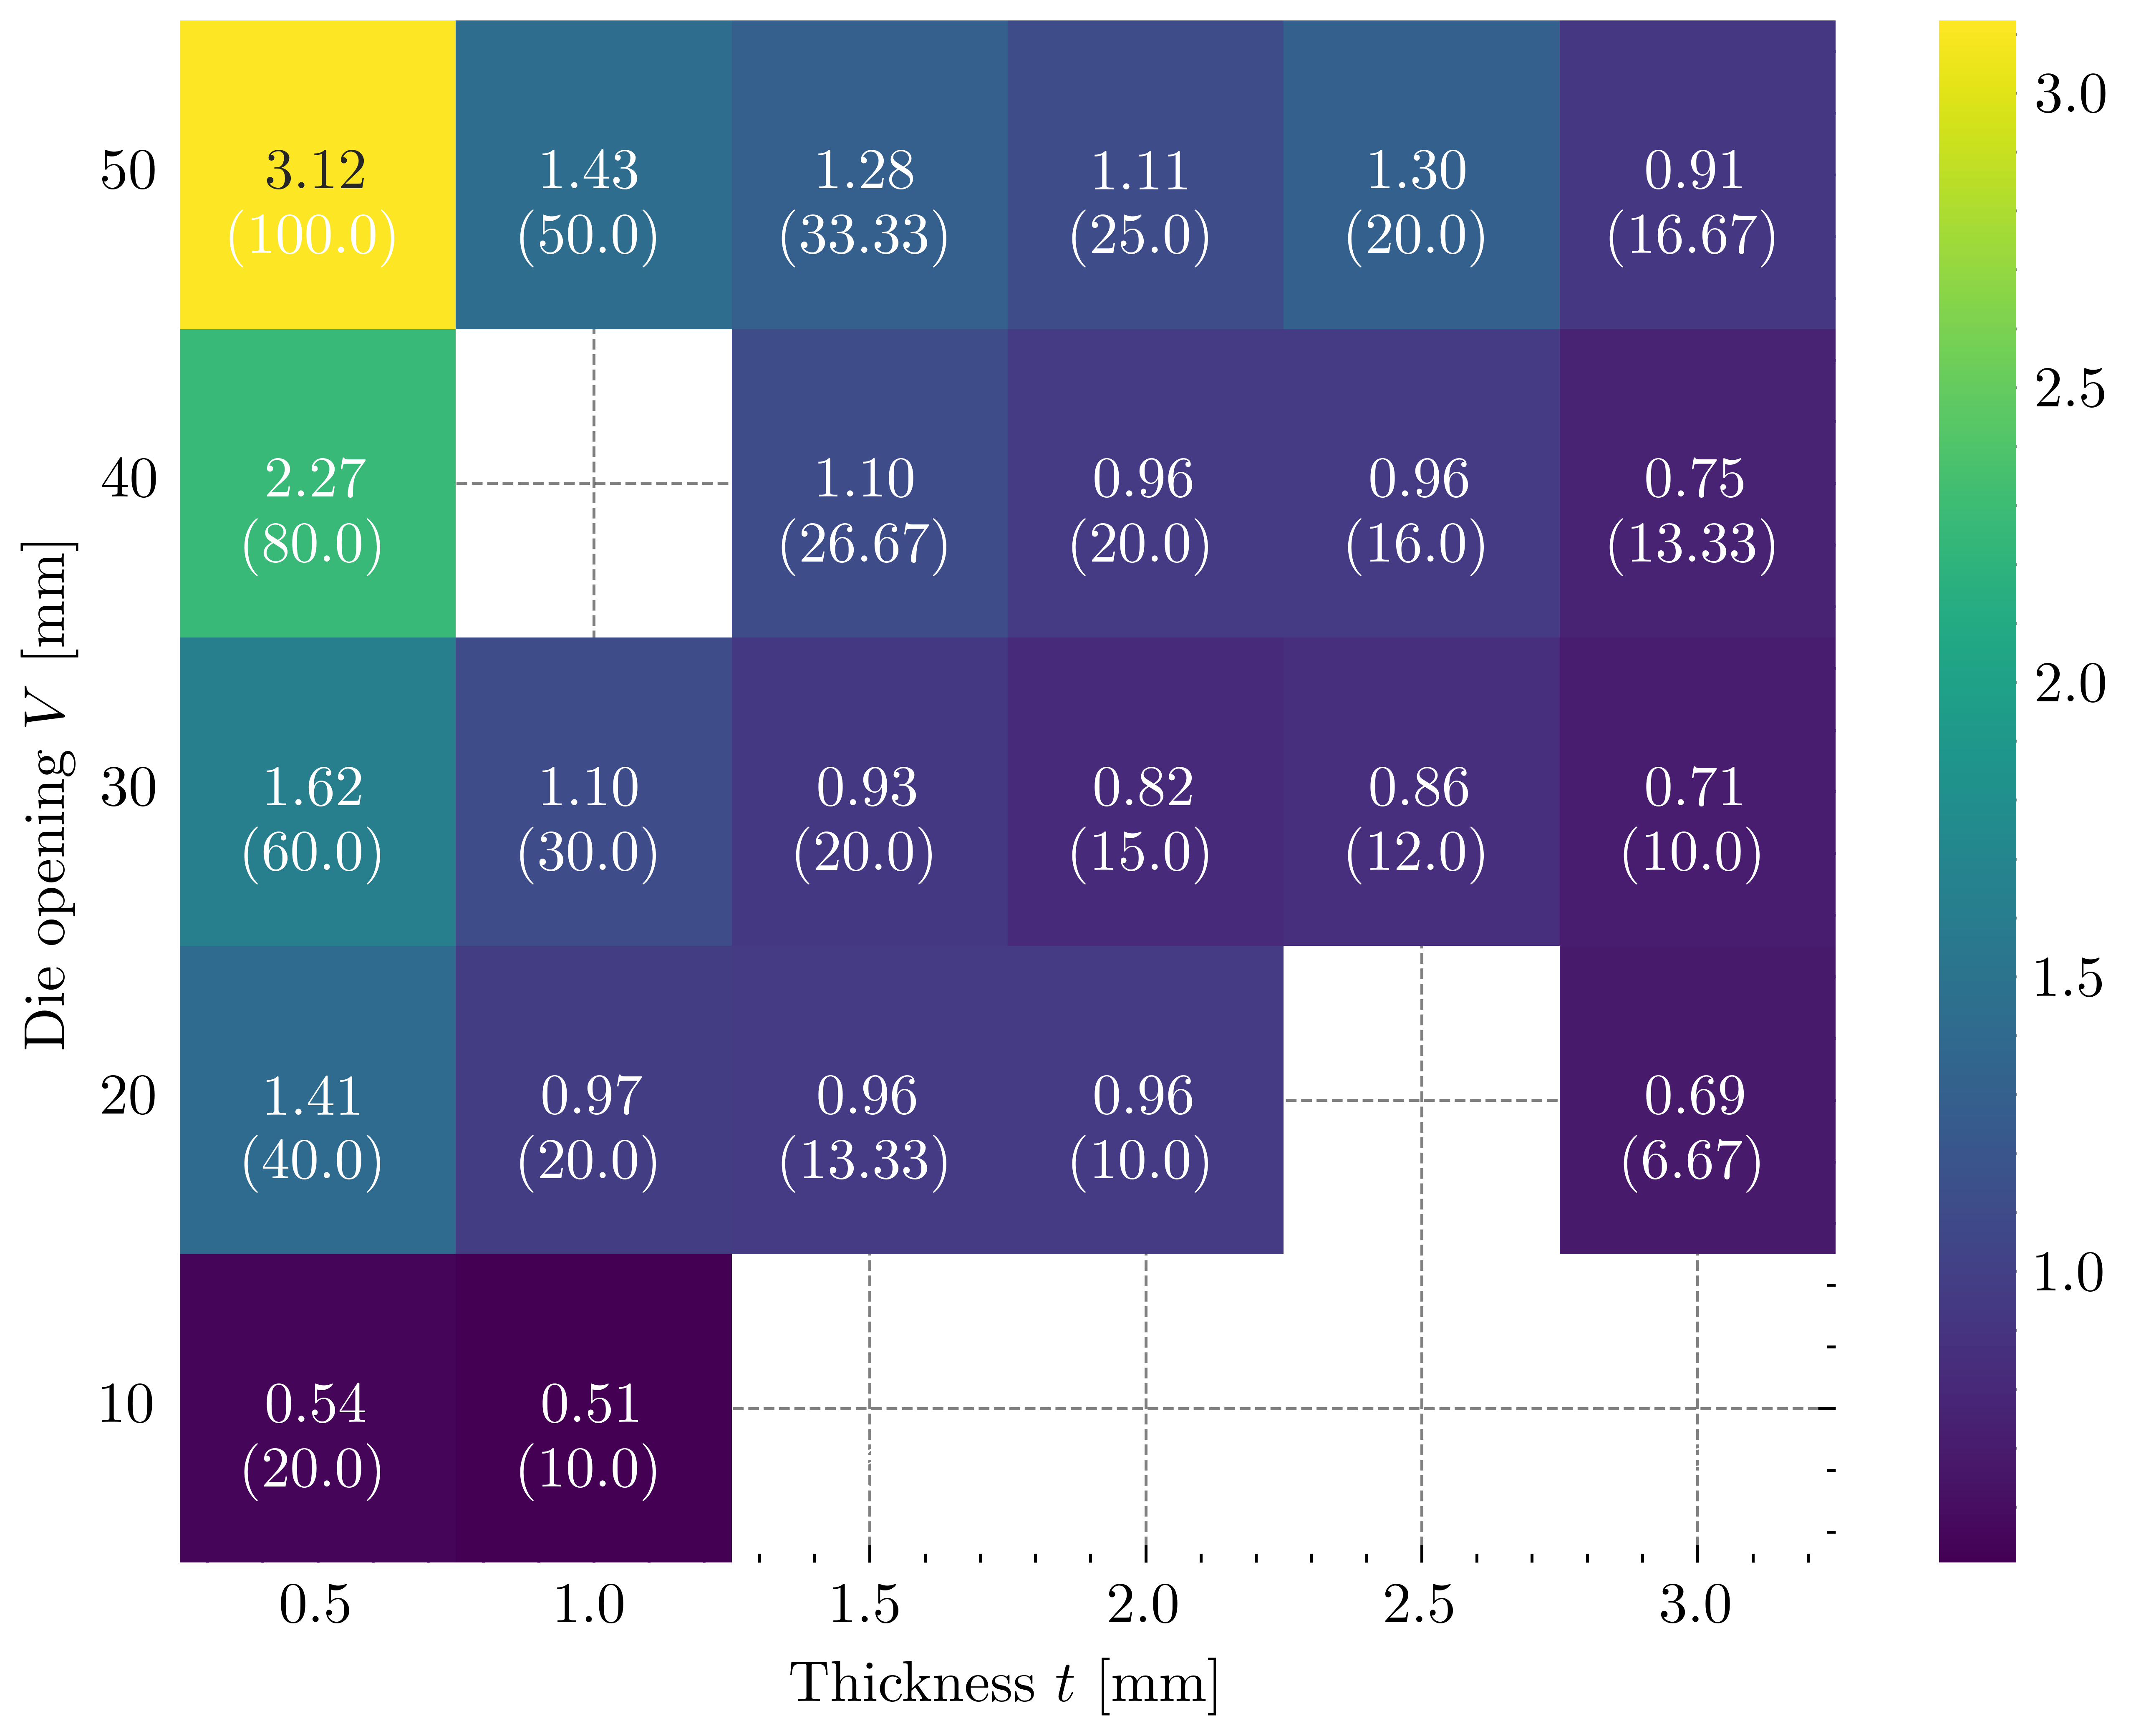
\includegraphics[width=0.8\textwidth]{chap5/images/mean_springback_heatmap}
    \end{tcolorbox}
    \caption{Feature importance of the random forest model.}
    \label{fig:springback-heatmap}
\end{figure}

To select specific instances for the demonstration, the V/t ratios of the instances are considered.
A V/t ratios around 20 is considered to in the middle of the the dataset.
Therefore three cases are defined, where the V/t ratios are below, within and above the recommended range.

The selected representative instances for the local methods are from one of three cases:
\begin{itemize}
    \item Case A includes instances with V/t ratios below the recommended range.
    \item Case B includes instances within the recommended range of V/t ratios.
    \item Case C includes instances with V/t ratios above the recommended range.
\end{itemize}

Chosen instances from each case are shown in Table~\ref{tab:representative-instances}.
The tabe shows the instances chosen grouped by the fact if there in, below or above the recommended range.

\begin{table}[h]
    \begin{tcolorbox}[arc=0pt,boxrule=0.5pt]
        \centering
        \begin{tabular}{lllll}
            \toprule
            \textbf{Case} & \textbf{\(V\) } & \textbf{\(t\)} & \textbf{V/t} & \textbf{In Range} \\
            \toprule
            A             & 20              & 3.0            & 6.66         & below             \\
            \hdashline
            B             & 30              & 1.5            & 20           & in                \\
%            B             & 20              & 1.5            & 13.33        & in                \\
            A             & 20              & 2.0            & 10           & in                \\
            \hdashline
            C             & 40              & 0.5            & 80           & above             \\
            C             & 50              & 0.5            & 100          & above             \\
            \bottomrule
        \end{tabular}
    \end{tcolorbox}
    \caption{Representative instances for the local methods.
    V denots the die opening, t denotes the thickness of the metal sheet and V/t denotes the V/t ratio.
    The last column indicates if the V/t ratio is in, below or above the recommended range.}
    \label{tab:representative-instances}
\end{table}

\subsection{Comparison of the Models}\label{subsec:overall-comparison-model-performance}
In this section, the outcomes generated by the trained models on the selected cases A, B, and C are presented. To
ensure unbiased results, all samples that were part of the test cases were removed from the training data set.
For instance, for case A(a), all samples with a die opening of 20 and a thickness of 2 were removed from the dataset.
This was done to prevent the models from overfitting to the test cases.
While it is anticipated that the models' performance may decline in these tests due to the removal of training data,
The decline is unlikely to be large.

It is vital to remember that the goal values represent the mean of all values when evaluating the numbers below.
While the dataset's quality is not perfect, there may \ e some outliers present.
In some circumstances, there are just a few samples for a particular sample, therefore the mean is not a reliable
reflection of the true value.


Figure~\ref{fig:performance-case-a} depicts two chosen test cases for case A with a V/t-ratio below the recommended
range.
Test case (a) performs quite well overall and all models can predict the spring back with a mean absolute error of
less than 0.5 mm.
The weak point of the model seems to be the predictions of the edge punch penetration values and it can be seen that
the predictions is always lower than the actual value.
However, the models' performance deteriorates in instance (b)\ref{fig:performance-20-3.0} with a V/t-ratio of 6.6,
particularly in the prediction of spring backs.

\begin{figure}[h]
    \begin{tcolorbox}[arc=0pt,boxrule=0.5pt]
        % Todo V20 t.2.5
%        \begin{subfigure}{0.5\textwidth}
%            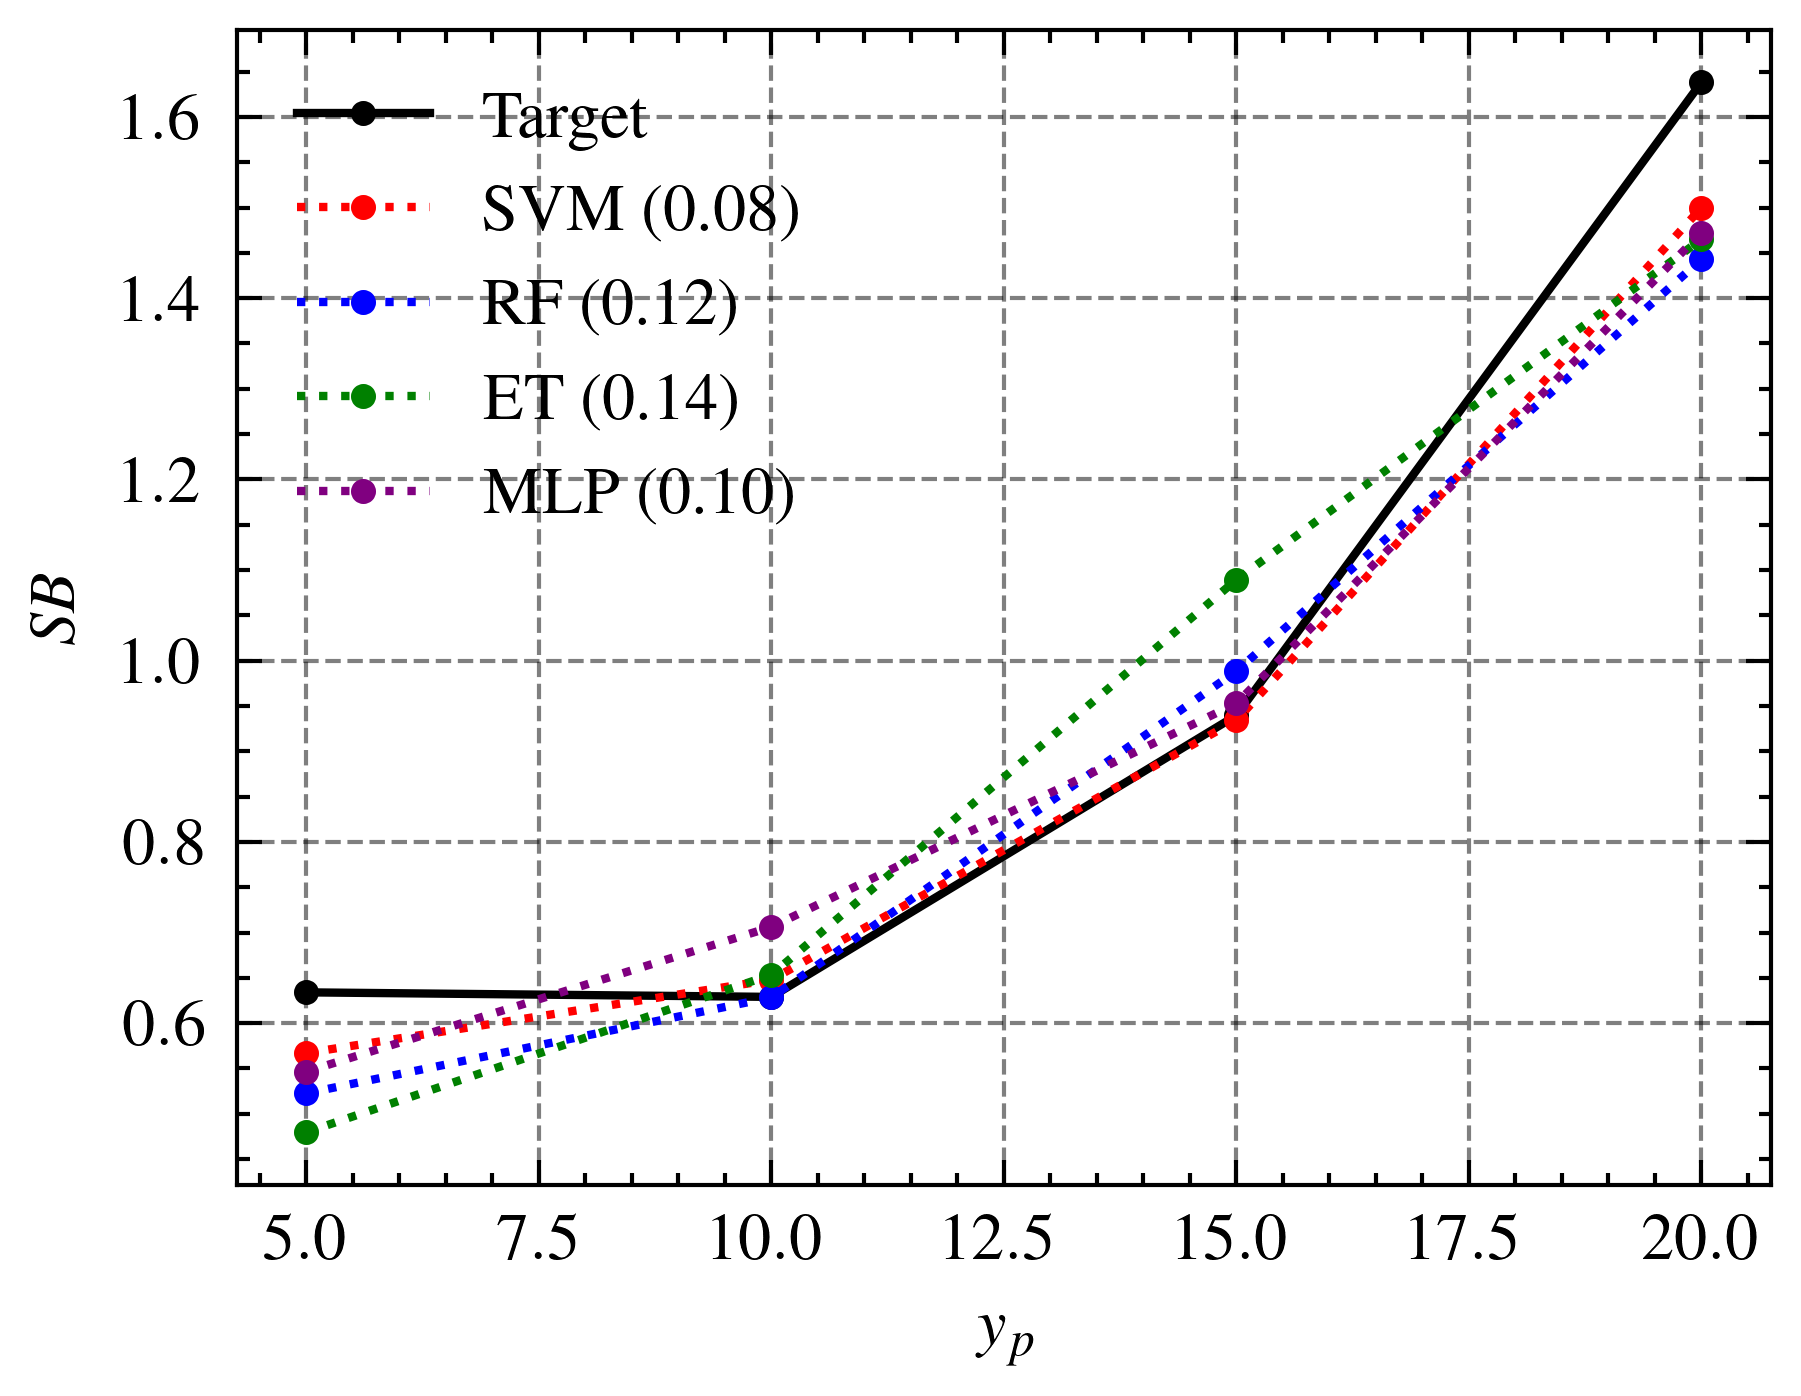
\includegraphics[width=\textwidth]{chap5/images/performance_20_2.0}
%            \caption{V: 20, t: 2}
%            \label{fig:performance-20-2.0}
%        \end{subfigure}
        \hfill
        \begin{subfigure}{0.5\textwidth}
            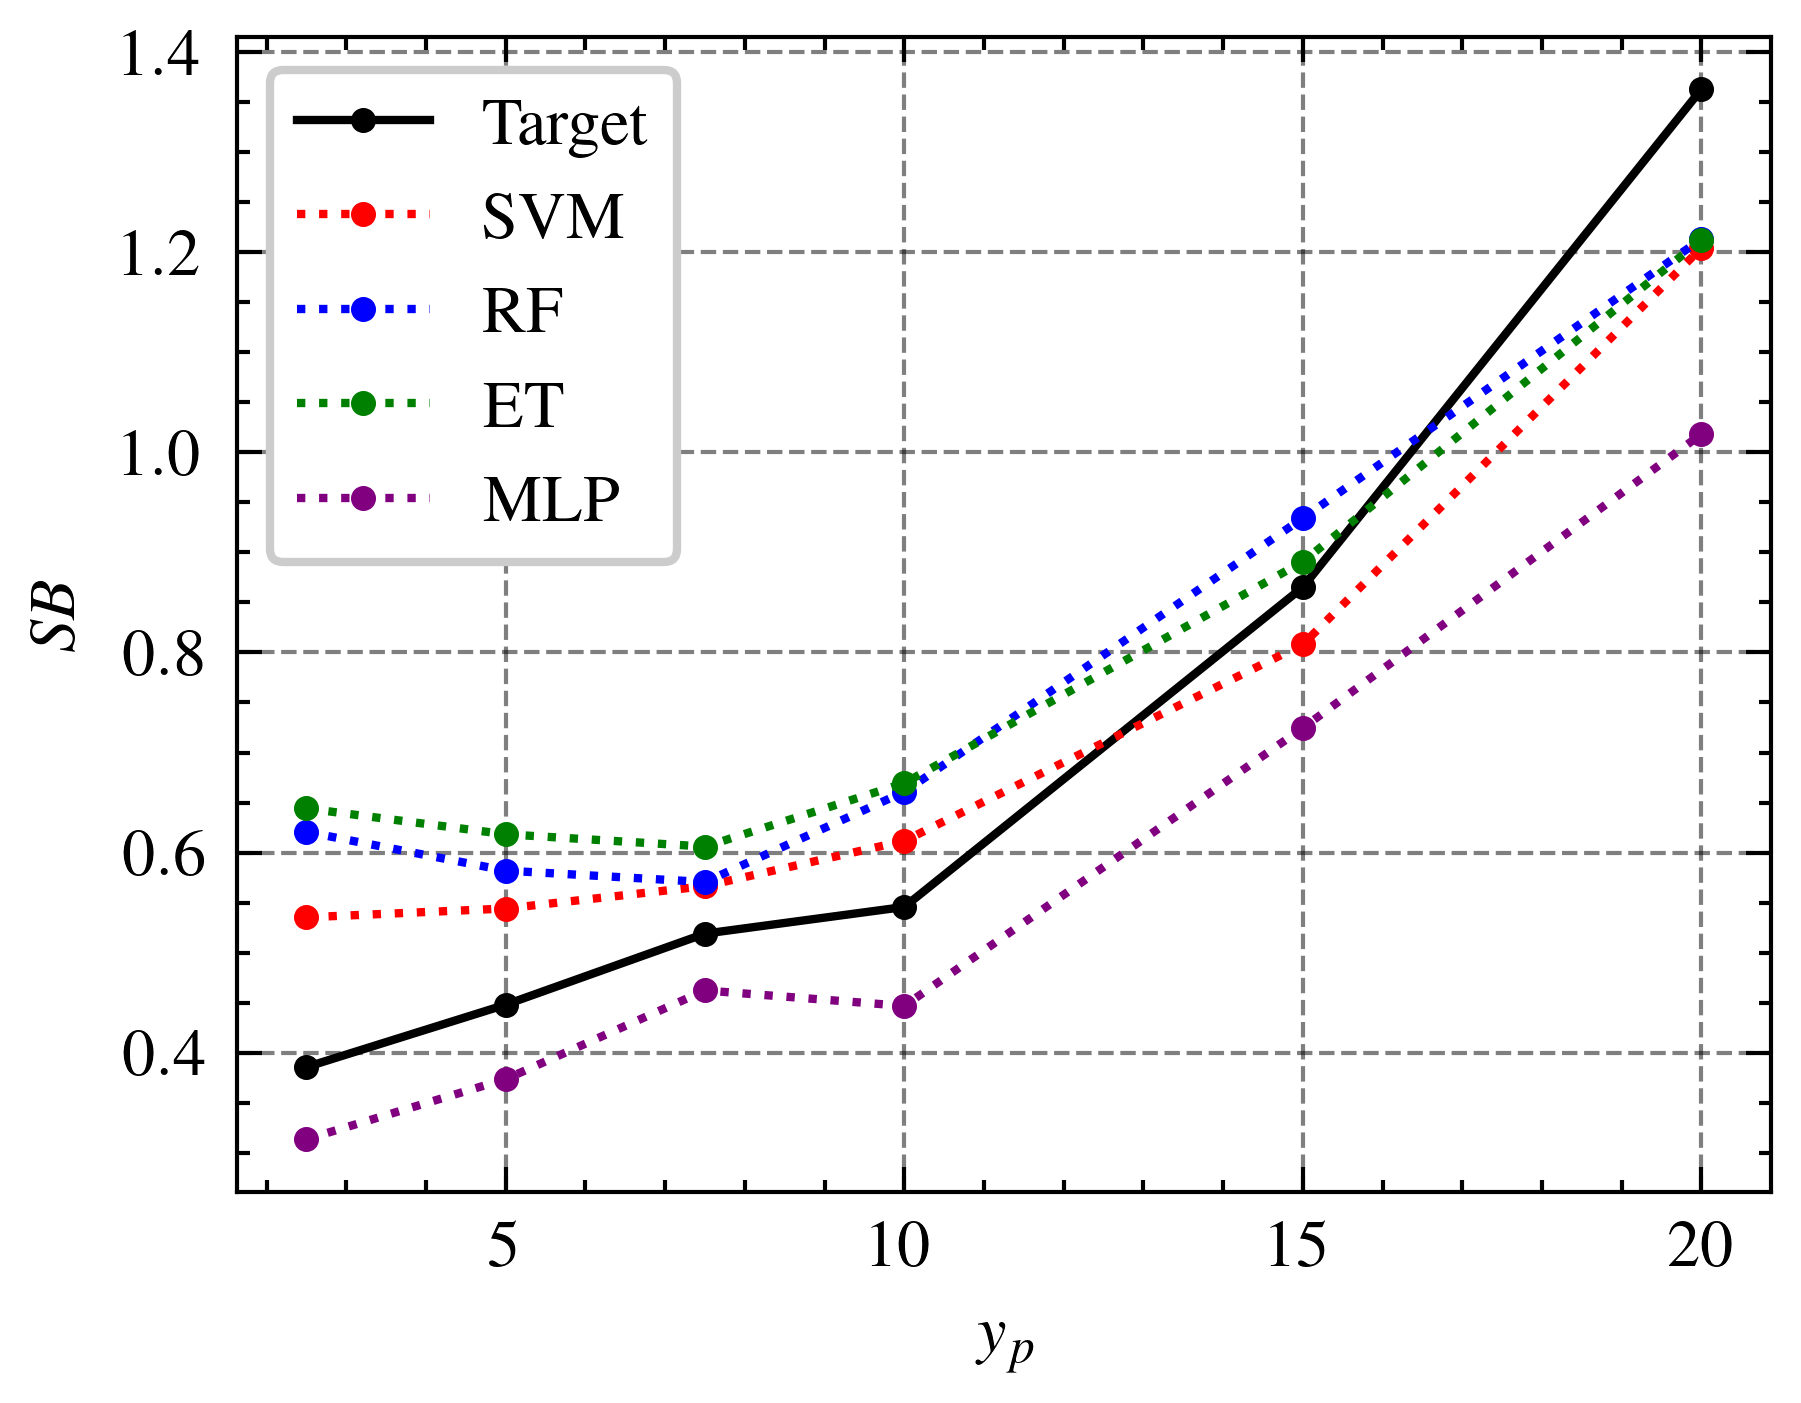
\includegraphics[width=\textwidth]{chap5/images/performance_20_3.0}
            \caption{V: 20, t: 3}
            \label{fig:performance-20-3.0}
        \end{subfigure}
    \end{tcolorbox}
    \caption{Performance plots for case A}
    \label{fig:performance-case-a}
\end{figure}

Figure~\ref{fig:performance-case-b} illustrates two selected test series for case B, where the V/t ratios fall within
the recommended range.
These test series produced the best results compared to cases A and C.
In instances (a) and (b), all models performed reasonably well, with instance (b) displaying better overall
performance.
It is apparent that the SVM model appears to predict spring back better in case (a), while the MLP model performs
best in case (b).
Overall, it is difficult to identify a clear favorite model based on the performance of the models in these test
series. Although some models performed better than others for specific variables or scenarios, the differences were
not significant enough to identify a clear winner. Therefore, the selection of an appropriate model will be
determined by the outcomes of the other two cases, A and C.

\begin{figure}[h]
    \begin{tcolorbox}[arc=0pt,boxrule=0.5pt]
        \begin{subfigure}{0.5\textwidth}
            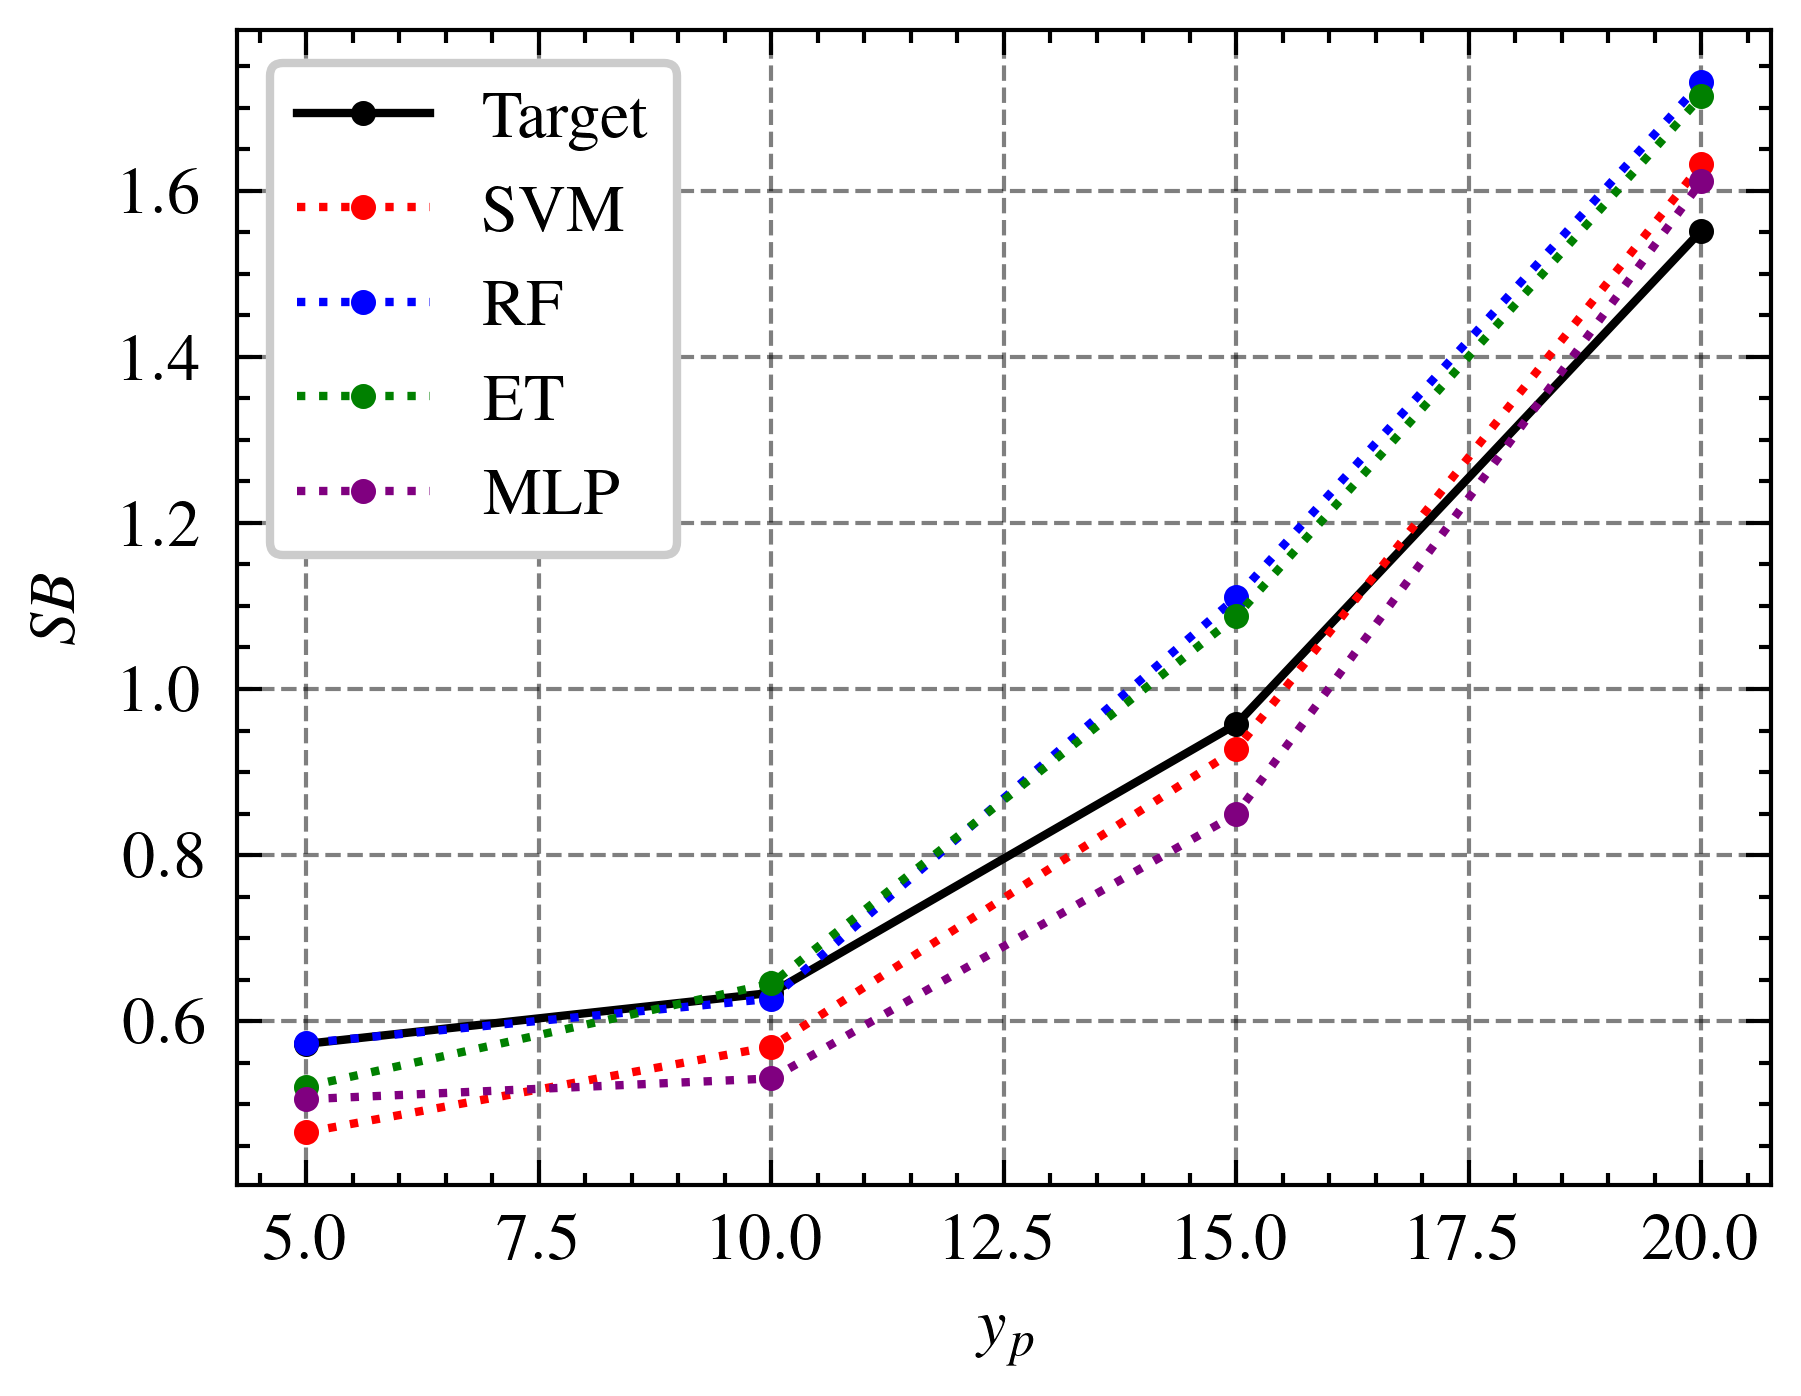
\includegraphics[width=\textwidth]{chap5/images/performance_20_1.5}
            \caption{V: 20, t: 1.5}
            \label{fig:performance-20-1.5}
        \end{subfigure}
        \hfill
        \begin{subfigure}{0.5\textwidth}
            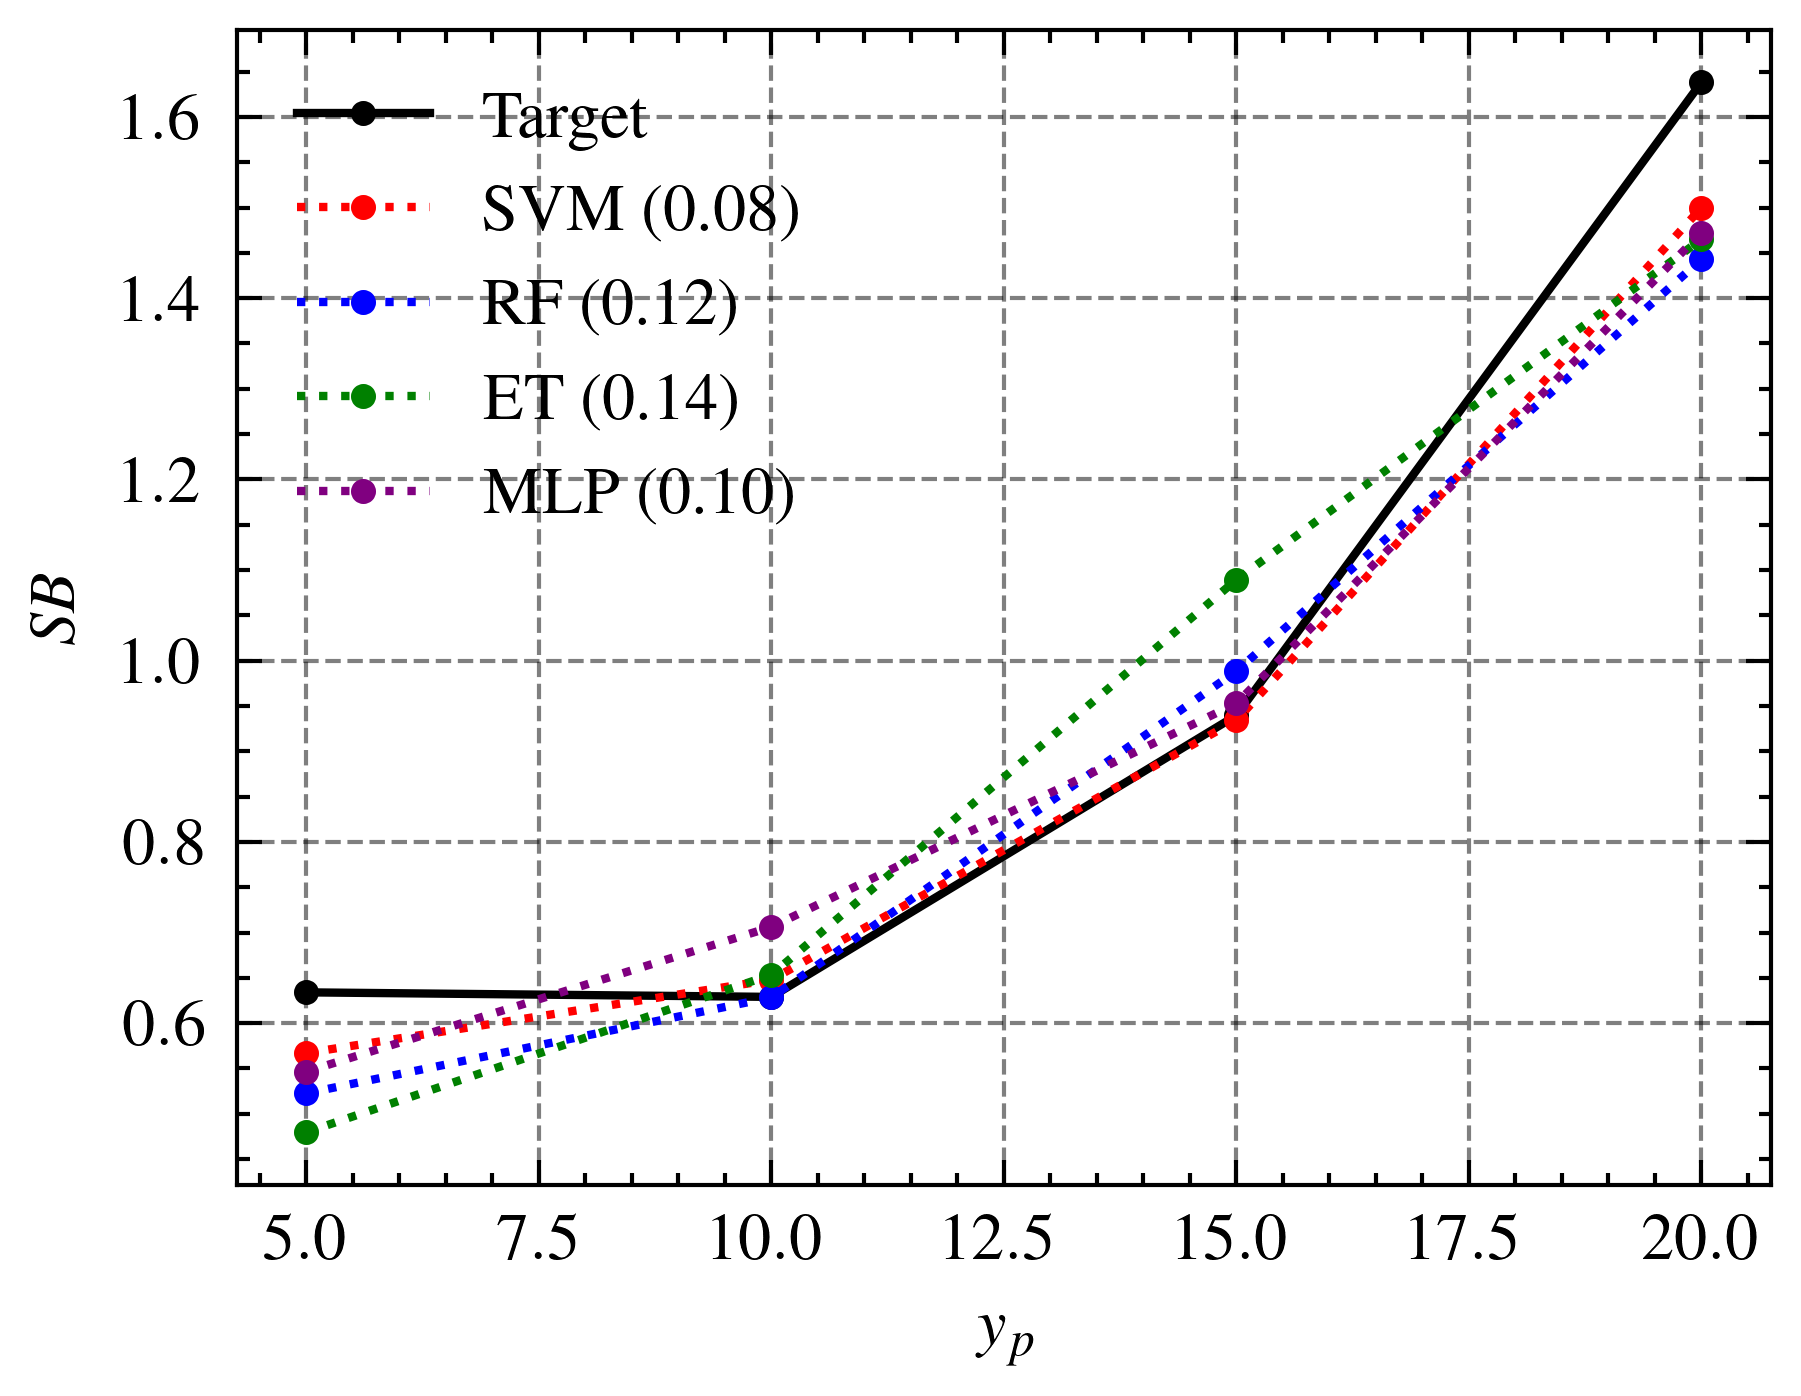
\includegraphics[width=\textwidth]{chap5/images/performance_20_2.0}
            \caption{V: 20, t: 2}
            \label{fig:performance-20_2.0}
        \end{subfigure}
    \end{tcolorbox}
    \caption{Performance plots for case B}
    \label{fig:performance-case-b}
\end{figure}

Case C is the most challenging case, as all models exhibit visibly poor performance. This is expected since the V/t
ratio is well above the recommended range.
The results are unusable, as the models are unable to predict the spring
back.
However, in Figure~\ref{fig:performance-50_1}, the results appear more promising, with the RF and SVM models
demonstrating the most consistent performance.
More work is clearly needed to construct machine learning models that perform well in these settings.

\begin{figure}[h]
    \begin{tcolorbox}[arc=0pt,boxrule=0.5pt]
        \begin{subfigure}{0.5\textwidth}
            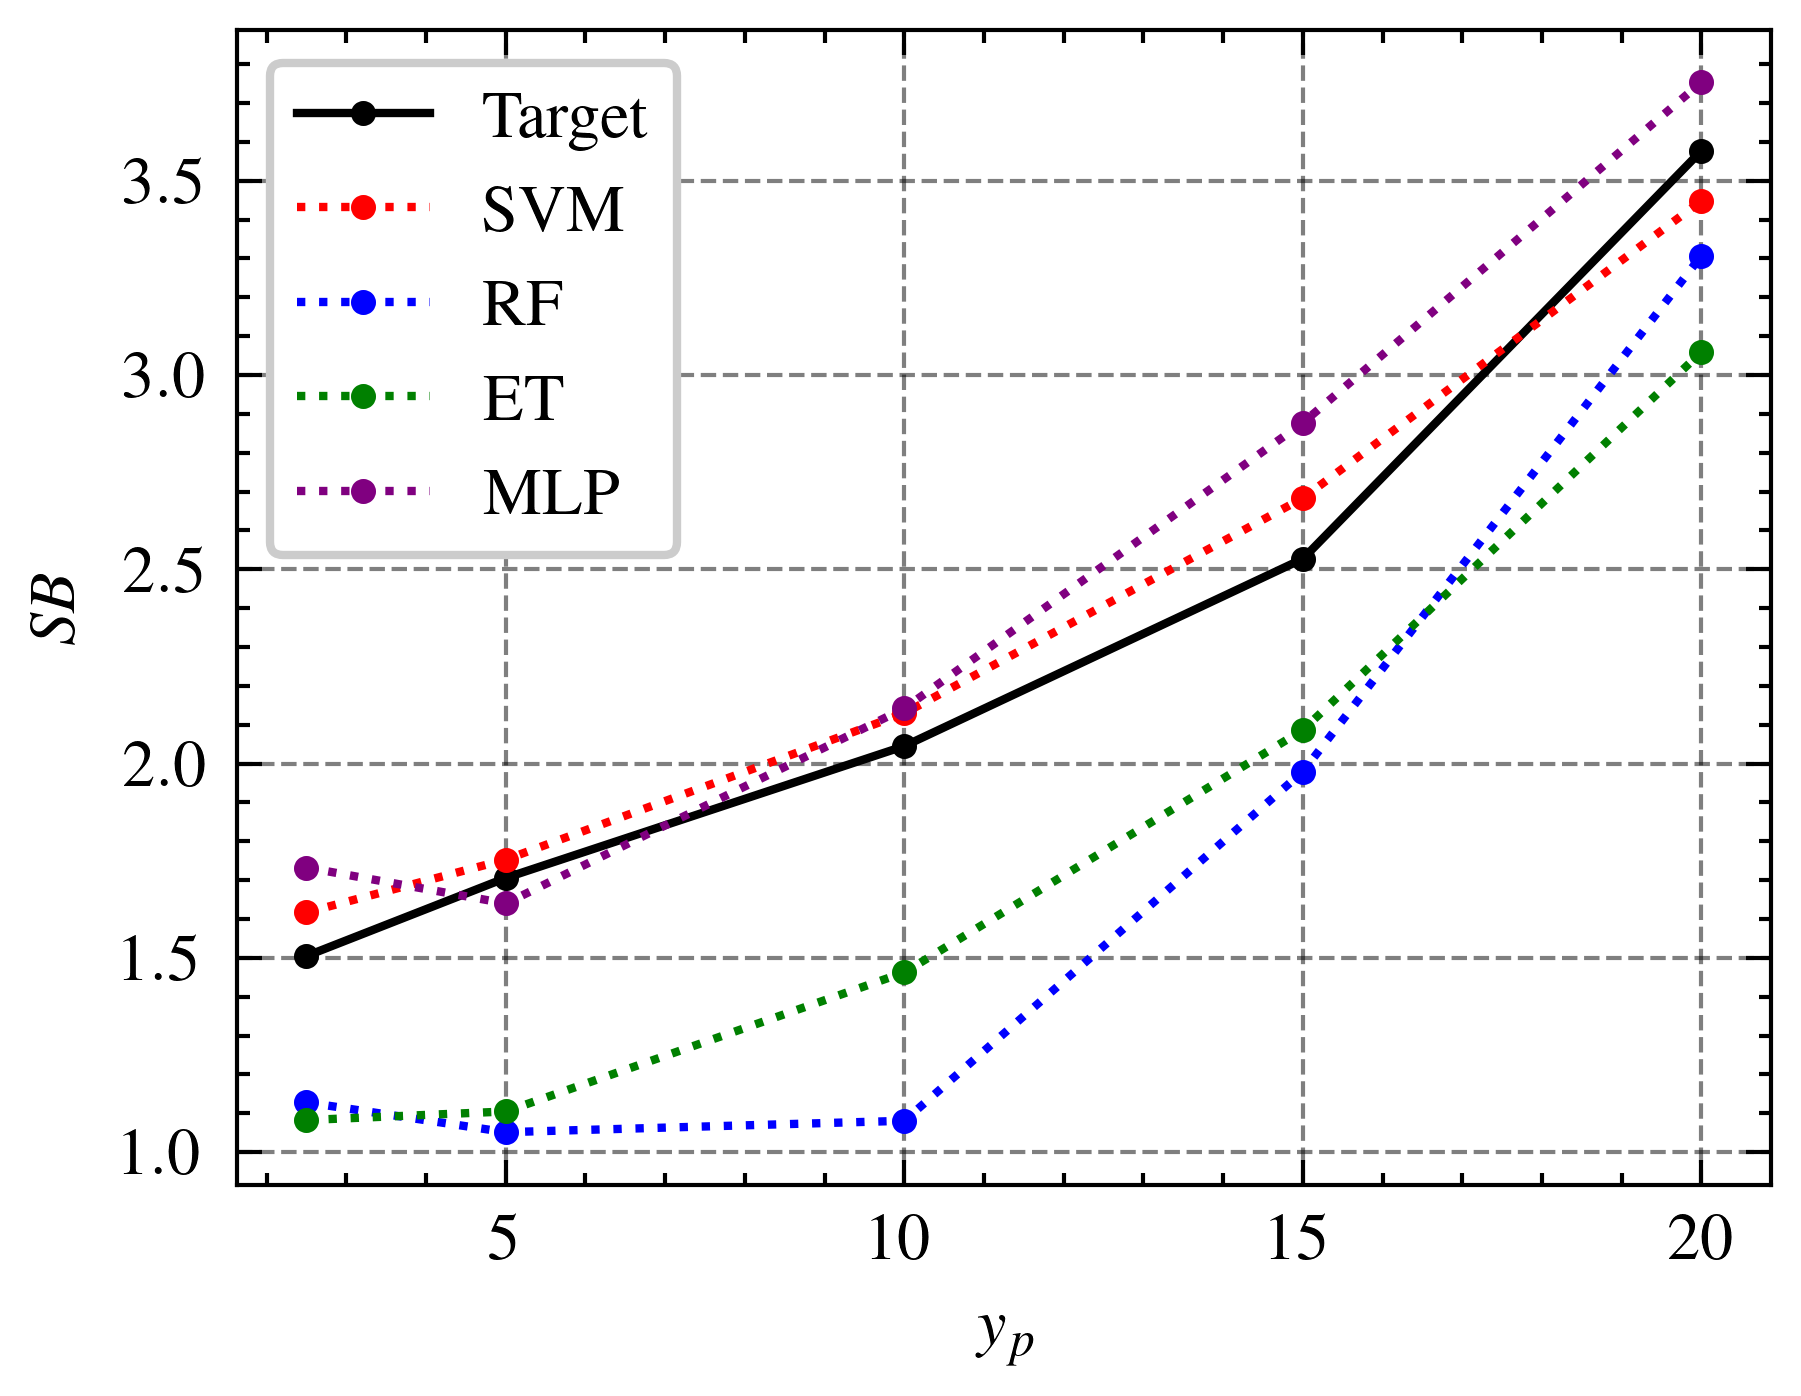
\includegraphics[width=\textwidth]{chap5/images/performance_40_0.5}
            \caption{V: 50, t: 0.5}
            \label{fig:performance-50_0.5}
        \end{subfigure}
        \hfill
        \begin{subfigure}{0.5\textwidth}
            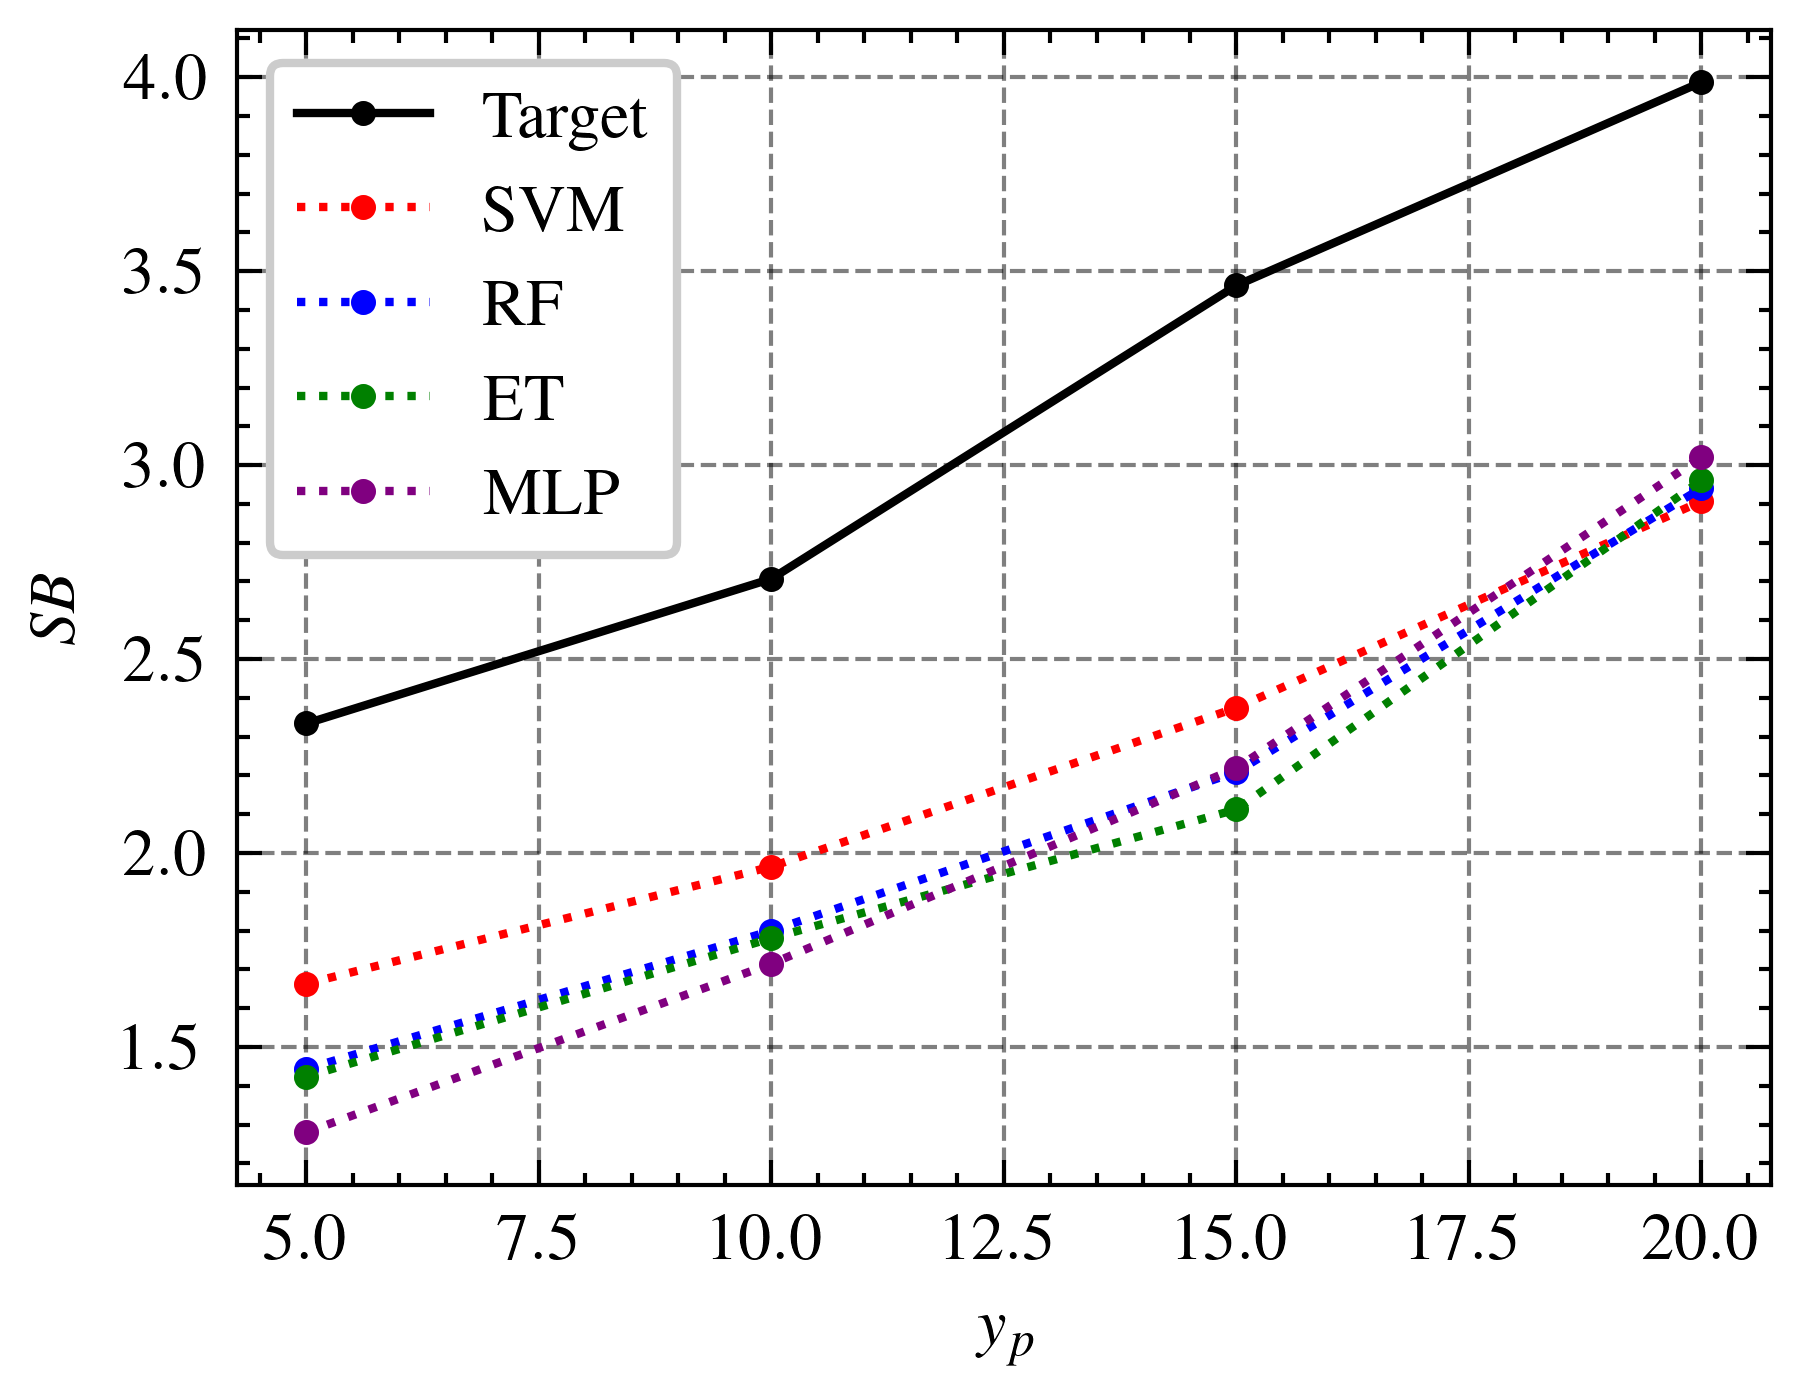
\includegraphics[width=\textwidth]{chap5/images/performance_50_0.5}
            \caption{V: 50, t: 1}
            \label{fig:performance-50_1}
        \end{subfigure}
    \end{tcolorbox}
    \caption{Performance plots for case C}
    \label{fig:performance-case-c}
\end{figure}

The best overall performing models are the \ac{MLP} and the \ac{SVM} model.
As seen before, the model performs consistent across all three scenarios, indicating that it can
effectively handle a broad range of V/t ratios also outside the recommended industry guidelines
range.
Therefore the chosen models for more detailed analysis are the \ac{MLP} and the \ac{SVM} model.

Overall it can be said that the models are able to predict the spring back with high accuracy.
For bad predictions the error is less than 0.25 mm, which is within the tolerance of the
most manufacturing processes (This it not true yet).


\section{Results and Discussion}\label{sec:results-and-discussion}
This component of the research is structured as follows:
The first section, titled ''Summary of Results,'' presents a succinct review of the study's findings. The second
section, ''Interpretation of Results,'' delves deeper into the findings and seeks to explain them.
Both parts are structured according to the three research questions formulated
in~\ref{sec:problem-identification-and-motivation}.

\subsection{Summary of Results}\label{subsec:summary-of-results}
%Introduction
The research objective of this study is to determine whether \ac{ML} models can accurately predict the spring back of
bent sheet metal parts.
Furthermore, the study aims to identify which model or ensemble of models performs the best.
Lastly, it seeks to utilize interpretable models to gain insights into the bending process.

%Data Collection and Preprocessing

This study aims to determine the accuracy of \ac{ML} models in predicting the spring back of bent sheet metal parts,
identify the best-performing model or ensemble of models, and gain insights into the bending process using
interpretable models.

The data was collected by using the air-bending process and measuring the spring back with the output data of the
press brake.
The dataset contained 400 samples, with punch penetration, die opening, and metal sheet thickness as
input features and spring back as the target feature.
The data quality was deemed good, requiring little data preprocessing.
With a complete dataset, no data imputation was necessary.
The data was normalized using different scalers from the sci-kit learn library.

%Key Findings

\subsubsection{Hypothesis 1}

The first research question is whether ML models can accurately predict the spring back of bent sheet metal parts.
Design Principle 1 (correctness) was used to test this hypothesis using the regression metric RMSE as the main
evaluation criterion.
The results showed that most ML models were able to predict the spring back with a RMSE of less
than 0.2 mm, indicating acceptable accuracy.
The Extra Trees and Support Vector Machine models performed best with a RMSE of 0.15 mm.
The AdaBoost, Random Forest, and Gradient Boosting models demonstrated moderate prediction
performance, while the performance of Linear Regression and Decision Tree models showed poor performance and
therefore were not considered for further analysis.

\subsubsection{Hypothesis 2}

\textbf{Hypothesis 2:} Specific ML models or combinations of models (e.g., ensemble methods) will yield better
performance
in terms of the six Design Principles (DPs) compared to other models.

The second research question examines whether specific ML models or ensemble models outperform other models.
Design Principles 2 to 5 were used to test this hypothesis.

\textbf{Relevance}

Relevance was evaluated by assessing the bias-variance tradeoff of all trained models, except Linear Regression and
Decision Tree, which were ruled out.
The results showed that Extra Trees, Multi-Layer Perceptron, and Random Forest models had the best balance between
bias and variance, and therefore were considered the most relevant.
Most models were able to explain the variance in the data.

\textbf{Robustness}

The robustness of various ML models is evaluated by examining their performance in the presence of
missing data and noise.

The experiments with missing data indicate that all models perform well when trained with 90\% of the data.
However,when trained with 50\% or less, the MLP and GBT models outperform others.
When trained on less data, the SVM and MLP models perform best and appear to be the most robust.

The models are also tested with added Gaussian noise to the training data.
The performance of all models deteriorates rapidly as noise increases, with the first 20\% of noisy data causing the
most significant decline.
The Extra Trees model exhibits the most robust performance, while the Gradient Boosted Trees and Random Forest models
also demonstrate similar resilience.
Interestingly, the high-performing SVM and MLP models underperform under these conditions, likely due to overfitting
or sensitivity to outliers.

The findings emphasize the importance of using robust models and preprocessing the data to eliminate noise and
outliers.
Additionally, it was found that already more than 10\% of noise can have a significant impact on the
performance of the models.


\textbf{Stability}

Stability was evaluated using Leave One Out Cross Validation (LOOCV).
The primary metric of the evaluation was the standard deviation of the cross-validation scores.
Here the results showed that the Gradient Boosting model was the most stable with a standard deviation of 0.183,
followed by the Extra Trees and Random Forest models.

Interestingly, the SVM and MLP models, which showed good results in other Design Principles, were less stable
compared to the other models in this case.
While stability is an important factor to consider, other aspects, particularly the generalization error (correctness
), should also be taken into account.

\textbf{Resource Utilization}
The resource utilization was evaluated using three key metric: Training time, prediction time and memory usage.
This metrics should be used to evaluated the how much computational resources the trained \ac{ML} models need.

The results indicate that the Extra Tree model and the Random Forest of 19.541 ms and 24.912 ms models had the shortest
training time compared to the other models.
The MLP model had by far the longest training time with over 16 seconds for the relatively small dataset of 400 samples.
Regarding the inference time the Gradient Boosting model was the fastest, while the MLP again was the slowest.
The RF and ET models demonstrated comparable inference times.

In terms of memory usage the MLP model was the most memory intensive model with 170 KB of memory usage.
The other model's memory usage was comparably low ranging from 157 KB to 159 KB.
The dataset's small size leaded less complex models and that contributed to the low memory usage.

\textbf{Hypothesis 3:} ML models with high interpretability can provide valuable insights into the factors that
contribute to spring back, potentially leading to better understanding of the underlying physical processes and
more effective compensation strategies.

To answer the third hypothesis model-agnostic methods were used to evaluate the interoperability, as model specific
method where not suitable since the used interpretable algorithm did not perform well.
Global method agnostic methods such as feature dependence and partial dependence plots where applied to the best
performing models.

Thickness, distance and die opening where all identified as important features for the prediction spring back with the
thickness of the metal sheet having the biggest influence on the outcome.
Partial dependence plots revealed non-linear dependencies between the features and the target variable.
Permutation feature importance and SHAP where sued to to further investigate the importance of the features.
The results indicated that thickness and punch penetration were crucial for the models decision-making while while the
die opening was important but only in combination with the other two features.
Two-way partial dependence plots showed an interaction between thickness and distance, confirming the importance of the
die opening for the predictions.

Also the model-agnostic method LIME was applied to different machine learning models but did not yield any new insights.

\subsubsection*{Further Results}
Additionally to the results found for the three hypotheses more insights where gained during the research process.
This study used the \ac{DSR} methodology to guide the research process as well as Design Principles as guidelines for
this process.
It is common for other research to use only regression metrics like MAE and RMSE for to evaluate the models.
This is understandable since the correctness of a models is usually the most important factor for the evaluation.
But these metrics alone do not provide a complete picture of the models performance, since they do not consider
other important factors like the interpretability of the model or the computational resources needed to train and
predict with the model.

This study attempted to create a more comprehensive framework for the evaluation of the models by using the Design
Principles as based on the IEEE ISO/IEC 9126 guidelines.
Until a similar standard is developed for \ac{ML} models this study provides a good starting point for future research
in this field.
This framework could be used in further research to evaluate the performance of \ac{ML} models not only in the field of
spring back prediction but also in other fields.

\subsection{Interpretation of Results}\label{subsec:interpretation-of-results}

The results of the this study provide insights in the applications of machine learning on the field of metal sheet
bending and the prediction of spring back.
The interpretation of the results is as follows:

\subsubsection{Hypothesis 1}
The findings support the first hypothesis that \ac{ML} models can accurately predict the spring back of bent sheet
metal parts.
The Extra Tree and Support Vector Machine models performed best with a RMSE of 0.15 mm, while other models still
exhibited good performance.
This means that in average the predictions of the best models derivative by 0.15 mm from the actual spring back,
with spring backs ranging from 0.5 mm to 3.1 mm in this study this performance is acceptable for many applications.

Traditional trial-and-error methods, such as technology tables (refer to
Section~\ref{sec:problem-identification-and-motivation}), offer data for a limited number of bends, encompassing
only those bends that were previously tested.
In contrast, the resulting \ac{ML} models from this study are capable of predicting an unlimited number of new bends
with high accuracy.
Therefore, it can be conclusively stated that \ac{ML} models are capable of outperforming traditional methods.

In the presentation section (see~\ref{sec:demonstration}) it could be seen that the models are not perfect.
In particularly they tend to underestimate high spring back values, this could be part of an area where further research
may be needed.
To improve the prediction accuracy more data for high spring back cases might already be enough to improve the to a
satisfying level.

The use of real-word data instead of simulated data for the training of the models make the results of this study more
representative for real-world applications.
A comparison with other studies is challenging since variations in the bending process such as material, machine,
bending method and other factors might yield significantly different results.
%In comparison with similar studies like \cite{baig_machinelearningprediction_2021} it can be seen that the
%real -world data used definitely paid of comparing the results

\subsubsection{Hypothesis 2}

The results show that specific \ac{ML} perform better compared to other models based on the six Design Principles
that where used.
The Extra Tree model demonstrated the best balance between bias and variance, as well as robust performance when
exposed to missing data and noise.
The Gradient Boosting model displayed the highest stability, while the Extra Tree and Random Forest models exhibited
the best resource utilization.
These findings suggest that selecting the most suitable ML models for specific applications is crucial for achieving
optimal performance.

The best overall performance was achieved by the Extra Tree model.
It was the only model that performed well in all performed tests.
The Extra Tree model is a good choice for applications where the model should be trained on a small dataset and
Should be able to accurately forecast new samples.
It is crucial to highlight that only a simple neural network was utilized in this study, and while it produced good
results, more complicated neural networks could produce even better outcomes.
Further more the use of ensemble models could yield interesting results (see recommendations for further
research~\ref{subsec:recommendations-for-further-research}).

\subsubsection{Hypothesis 3}
The results show interpretability methods can provide valuable insights into factors that contribute to spring back,
potentially leading to a better understanding of the underlying physical processes and more effective compensation
strategies.
The thickness of the metal sheet was found to have the most significant influence on spring back, while other
features, such as punch penetration and die opening, also played important roles in the models' decision-making
processes.

With he use of model-agnostic methods, the study also revealed non-linear dependencies between the input and the
target features, as well as interactions between thickness and distance.
This information can be valuable for further refining the models, as well as for developing more effective
compensation strategies in the sheet metal forming process.
This study was not able to use models with high interpretability such as decision trees or linear models
since their performance was not good enough.

\subsection{Limitations of Research}\label{subsec:limitations-of-research}
There are some limitations to this studay that needed to be considered when interpreting the results.

The dataset used has a limited number of samples, with 400 samples the models might not have enough data to capture
the full complexity of the spring back phenomenon.
Furthermore the dataset did not contain many high spring back scenarios, which might have led to the models
underestimating high spring back values.
A larger dataset with more high spring back samples could potentially improve the model performance.
Additionally it has to be noted that many parameters weren't changed in the experimental setup.
For example the used press brake, punch radius and material of the metal sheets where not changed.
Experiments with different bending methods and materials will most certainly yield different results.

This study had a limited number of input features (punch penetration, die opening and
metal sheet thickness).
Other potentially relevant factors such as material properties, temperatures might limited the models ability to
capture all factors affecting the spring back.

Also this study had to selected a limited number of models,
there might be other models or more advanced techniques that might yield better results, recommendations for further
research will be made in the following section.

\subsection{Recommendations for Further Research}\label{subsec:recommendations-for-further-research}
The limitations identified in this study provide direction for future research.

This study selected a limited number of \ac{ML} methods, but there are other models that could be used to
predict spring back.
Based on the results, the \ac{MLP} demonstrated superior performance in multiple design principles, indicating that
deep learning models may be promising candidates for future research.
Furthermore using ensemble models that combine the strengths for multiple other models using bagging or stacking could
lead to interesting new results.
This would involve training multiple other models on the same dataset and combine their predictions to improve the
prediction performance and the robustness of the models.
Additionally the dataset could be expanded by adding more samples with high spring back values.
A larger dataset could potentially improve the model performance.

One of the most interesting directions for future research is the use of \ac{ML} models to predict bend deduction.
Bend deduction is the phenomenon where the metal sheet shrinks during the bending process, resulting in a smaller
piece than the one specified in the design.
Similar to the spring back this can lead to fitting issues and is therefore an important topic for further research.
As noted by~\cite{strano2017fusion}, while some predictions models are available for spring back, bend deduction is
frequently overlooked and could be a fruitful topic for future investigation.

Moreover there are likely other factors that influence the spring back beyond those included as features in this study.
To account for these additional patterns, future research could consider including features such as rolling
direction, temperature, and tension.
